\documentclass[12pt]{article}
\usepackage[utf8]{inputenc}
\usepackage[margin=1.0in]{geometry}
\usepackage{graphicx}
\usepackage{amsmath}
\usepackage{fancyhdr}
\usepackage[font={small,it}]{caption}

\title{\vspace{-1em}A Statistical Analysis of the Extreme Properties of the IMF and the Solar Wind}
\author{Benedek Kovács\\ Supervisor: Prof. Jim Wild}
\date{} 

\begin{document}
\pagenumbering{roman}
\newgeometry{margin=1.3in}
\maketitle
\begin{center}
        \makebox[\textwidth]{
\includegraphics[width=0.7\textwidth]{fig_other/LU_Logo_Physics.jpg}}
\end{center}
\bigskip
\begin{abstract}
    \noindent The 1859 Carrington Event is the strongest geomagnetic storm ever recorded. This study estimates how often a geomagnetic storm comparable to the 1859 Carrington Event or the 2003 Halloween Storms would return (return period), while setting up relations, that can be used to estimate how often certain strengths of the Interplanetary Magnetic Field, solar wind speed and solar wind ram pressure would return. The return period of the Carrington Event was estimated to be between $R\approx 21\, years$ and $R=317\, years$, suggesting that the simulations and estimations resulting in the IMF strength and solar wind speed values may be underestimating the actual values. The return period of the Halloween Storms was estimated to be $R=201\ years$. These results were achieved after analysing $\sim 20$ years of magnetic field and solar wind measurements, taken by the ACE satellite between the Earth and the Sun, at the Lagrange L1 point. To analyse the data, it was separated based on solar magnetic activity level and Generalised Extreme Value Distributions were fitted onto the daily maxima (minima) of the data. Finally, to set up relations between the return period and the return level, the parameters of these distributions have been estimated.
\end{abstract}
\newpage
\restoregeometry
\tableofcontents
\newpage
\pagestyle{fancy}
\fancyhf{}
\rhead{Benedek Kovács}
\lhead{\leftmark}
\cfoot{\thepage}
\pagenumbering{arabic}

\section{Introduction}\label{sec:introduction}
    \subsection{Space Weather Effects}\label{sec:spaceweather}
        Geomagnetic storms are causing a larger and larger headache, as humanity becomes more and more reliant on electricity. In the last approximately 30 years, geomagnetic storms caused at least two major and several minor disturbances, both on the surface of Earth and in satellites. During the storm of 1989, the Hydro-Québec power-system experienced a major blackout, with other, mostly North American countries affected by it as well\cite{1989hydroquebec}. In 2003, the `Halloween Storm' \cite{2003halloweensweden} caused power outages in Sweden and damaged or completely incapacitated several satellites. Recently, in February 2022, a smaller geomagnetic storm impacted several satellites in low-Earth orbit\cite{2022spacex}.\\ \\
        This report aims to study the properties of the solar wind and the Interplanetary Magnetic Field to infer the possibilities and probabilities of the events mentioned above happening again. This can help in forecasting these events and preventing, or at least limiting the damage caused by them. The main outcomes of this report are estimations of the relationships between return levels and return periods for the Interplanetary Magnetic Field, solar wind velocities and solar wind ram pressures in Section \ref{sec:returnperiod}. Further discussion of these topics and their relations to the return periods of an event similar to the Carrington Event or the 2003 Halloween Storms are examined in Section \ref{sec:carrington} and Section \ref{sec:halloween}.
    \subsection{Previous Studies}\label{sec:prevstudies}
        Previous studies often examine the patterns in solar wind data, but most of the time, these studies only investigate the trends and the fairly common data points, not the extremely small/large or the extremely rare data points. Russell's tutorial on solar wind and the Interplanetary Magnetic Field\cite{2001russell} includes several useful graphs and histograms describing solar wind and the IMF. This includes histograms showing the distribution of magnetic field strength at 1 AU distance from the Sun, which can be seen on Figures \ref{fig:russellBX}, \ref{fig:russellBY} and \ref{fig:russellBZ}. These histograms are helpful at showing the trends and usual data points, but lack depth at showing data points of extremely small or large IMF strength, as they seem to have a minimum and a maximum cut-off, due to the scaling of the graphs.\\
        \begin{figure}[t!]
            \begin{minipage}{0.48\textwidth}
                \centering
                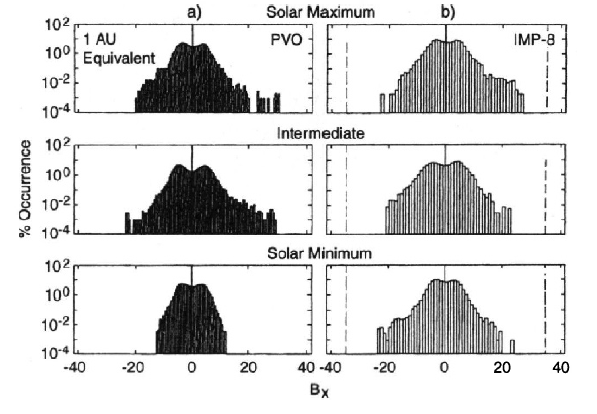
\includegraphics[width=\textwidth]{fig_introduction/russellBX.png}
                \caption{Histograms of the x-component of the Interplanetary Magnetic Field ($B_x$) at a distance of 1 AU from the Sun\cite{2001russell}. The data has been divided into 3 separate batches, based on the solar activity level at the time of measurement. 2 different data sets have been used (PVO 10-minute data on the left and IMP-8 5-minute data on the right). Measurements taken between 1978 and 1988.}
                \label{fig:russellBX}
            \end{minipage}
            \hfill
            \begin{minipage}{0.48\textwidth}
                \centering
                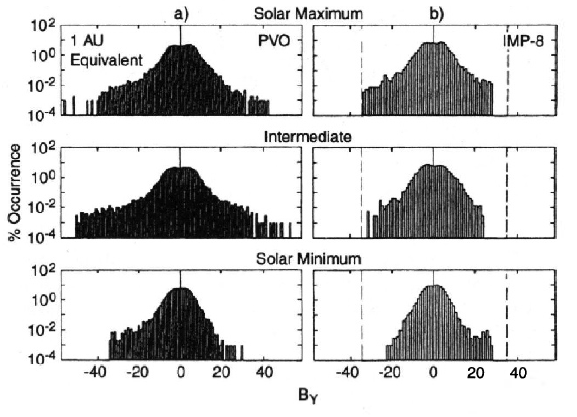
\includegraphics[width=\textwidth]{fig_introduction/russellBY.png}
                \caption{Histograms of the x-component of the Interplanetary Magnetic Field ($B_y$) at a distance of 1 AU from the Sun\cite{2001russell}. The data has been divided into 3 separate batches, based on the solar activity level at the time of measurement. 2 different data sets have been used (PVO 10-minute data on the left and IMP-8 5-minute data on the right).Measurements taken between 1978 and 1988.}
                \label{fig:russellBY}
            \end{minipage}
        \end{figure}
        \begin{figure}[t!]
            \centering
            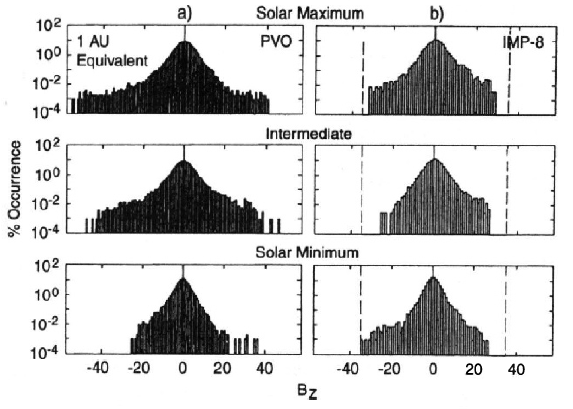
\includegraphics[width=0.48\textwidth]{fig_introduction/russellBZ.png}
            \caption{Histograms of the z-component of the Interplanetary Magnetic Field ($B_x$) at a distance of 1 AU from the Sun\cite{2001russell}. The data has been divided into 3 separate batches, based on the solar activity level at the time of measurement. 2 different data sets have been used (PVO 10-minute data on the left and IMP-8 5-minute data on the right).Measurements taken between 1978 and 1988.}
            \label{fig:russellBZ}
        \end{figure}\\
        It is important to note, that in the following sections, solar wind velocity and magnetic field strength in the x-direction will often be negative. This is due to the fact that the positive x-direction of the GSM coordinate system points from the Earth towards the Sun, therefore solar wind blowing from the Sun will be represented with a negative number, therefore the smaller (more negative) quantities will generally be considered stronger. The GSM coordinate system defines\cite{2017laundal} the positive x-coordinate to be pointing from the centre of the Earth towards the centre of the Sun, the positive y-coordinate to be the cross-product of the x-axis and the Earth's magnetic dipole axis, pointing towards the dusk side of the Earth. The z-coordinate is the cross-product of the x-axis and the y-axis, with the centre of the Earth at the origin of the GSM coordinate system.
\section{Background Theory}\label{sec:theory}
    \subsection{Properties of Solar Wind}\label{sec:solarwind}
        In 1958, Eugene Parker predicted the existence of solar wind\cite{1958parker}. 8 decades later we understand the solar wind a lot better and use modern equipment (e.g. satellites) to measure its properties and the magnetic field brought along with it.\\ \\
        Today, we understand that solar wind is made up of plasma, overwhelmingly composed of electrons and hydrogen nuclei (protons). Solar wind also contains heavier ions in the shape of heavier nuclei (mostly alpha particles), but the overwhelming majority of the solar wind is made up of electrons and protons (approximately 2.5\%-3.6\% of the solar wind consists of helium ions\cite{2006schwenn}). In this report, a composition of 50\% protons and 50\% electrons was assumed. This assumption was important for the calculations related to the solar wind ram pressure later in this report. Even though the solar wind is made up of charged particles, on large scales, it is considered neutral, therefore it is called quasi-neutral\cite{2007meyer}. This shows that it is approximately made up of equal number of positively and negatively charged particles.\\
        \begin{table}[t!]
            \begin{center}
                \begin{tabular}{|l|c|c|} \hline
                    &\textit{Slow Solar Wind}&\textit{Fast Solar Wind}\\ \hline
                    Origin&Open magnetic field lines&Coronal holes\\ \hline
                    Speed, $v_p$ ($km\ s^{-1}$)&250-400&400-800\\ \hline
                    Proton Density, $n_p$ ($cm^{-3}$)&10.7&3.0\\ \hline
                    Proton Temperature, $T_p$ ($K$)&$3.4\times 10^4$&$2.3\times 10^5$\\ \hline
                    Electron Temperature, $T_e$ ($K$)&$1.3\times 10^5$&$1\times 10^5$\\ \hline
                    Composition, $n_\alpha /n_p$ ($\%$)&$2.5$&$3.6$\\ \hline
                \end{tabular}
                \caption{A comparison between basic properties of slow and fast solar wind at 1 AU.\cite{2006schwenn} \label{tab:slowfast}}
            \end{center}
        \end{table}\\
        There are two different types of solar wind, which are different from each other to a great extent in their origin and other properties: the slow solar wind and the fast solar wind. Table \ref{tab:slowfast} shows the basic properties of slow and fast solar wind. The most important of these differences are their origin and their their velocity.\\ \\
        Although the exact origins of solar wind is still not understood completely, it is known that slow solar wind originates from open magnetic field lines in the Heliosphere. Due to Alfvén's theorem\cite{1976alfven}, the solar wind plasma flows along magnetic lines (and magnetic field lines follow the flow of plasma), hence it can move away from the Sun along open magnetic field lines. Conversely, fast solar wind originates from coronal holes, which are dense regions of open magnetic field lines. The stronger magnetic field in these regions allows solar wind to escape at a higher rate and higher velocity. Coronal holes are mostly unpredictable and temporary, therefore it is hard to forecast their activity.\\ \\
        The second main difference between slow and fast solar wind is their velocity. The variance in the velocity of the slow solar wind is fairly low, between $250\,$km/s and $400\,$km/s. This is most likely due to the reliable and constant nature of its origin. Contrarily, the variance in the velocity of the fast solar wind is fairly high, between $400\,$km/s and $800\,$km/s, although rarely it does flow even faster that.
    \subsection{Solar Magnetic Activity Cycle}\label{sec:solarcycle}
        Solar cycles are approximately 11-year long cycles, during which the north pole and the south pole of the Sun switch around. This happens during maximum solar activity (or more accurately, maximum solar activity happens, when the poles of the Sun switch around). The solar activity level (and hence the properties of the cycle itself) are measured by counting the number of sunspots visible on the surface of the Sun. Figure \ref{fig:sunspots} shows the average number of sunspots counted, beginning around 1750. The graphs clearly show a periodicity in the average number of sunspots counted, with a period of approximately 11 years. It is also important to note, that the maximum of every period can extremely differ from each other (e.g. the maximum average sunspot number in Solar Cycle 5 was around 70, while in Solar Cycle 19 it was around 250).\\
        \begin{figure}[t!]
            \centering
            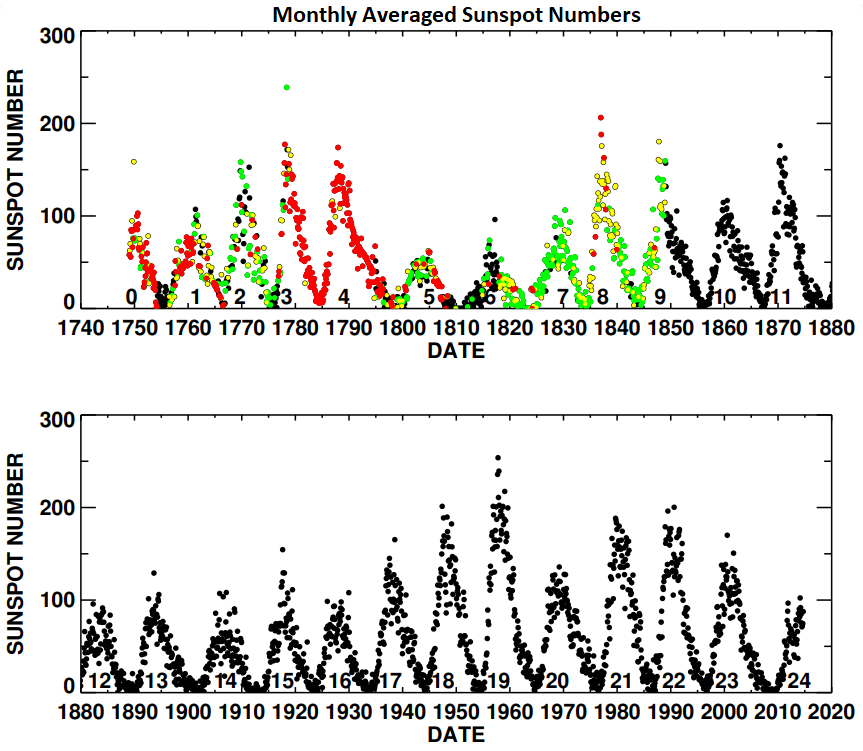
\includegraphics[width=0.8\textwidth]{fig_theory/sunspots.png}
            \caption{The monthly averaged sunspot numbers. Red: more than 20 days of observations missing per month. Yellow: between 11 and 20 days of observations missing per month. Green: between 1 and 10 days of observations missing per month. Black: no observations missing. The numbers above the horizontal axis indicate the number of the solar cycle. An 11-year cycle is clearly visible, as approximately 11 year go by between the spikes. Source: \cite{2015hathaway}}
            \label{fig:sunspots}
        \end{figure}\\
        The solar cycle impacts the number of coronal holes in the corona of the Sun in an unexpected way. Since coronal holes are the primary source of fast solar wind, it is reasonable to assume, that higher solar wind speed measurements are due to more/larger coronal holes. Interestingly, Figure \ref{fig:sw_speeds} show in increase in solar wind speed during the decline to (e.g. 1994) and during the minimum activity periods (e.g. 1986)\cite{2010tokumaru}. This effect is also visible in form of the spike on the top left histogram on Figure \ref{fig:hist_sw}.\\
        \begin{figure}[t!]
            \centering
            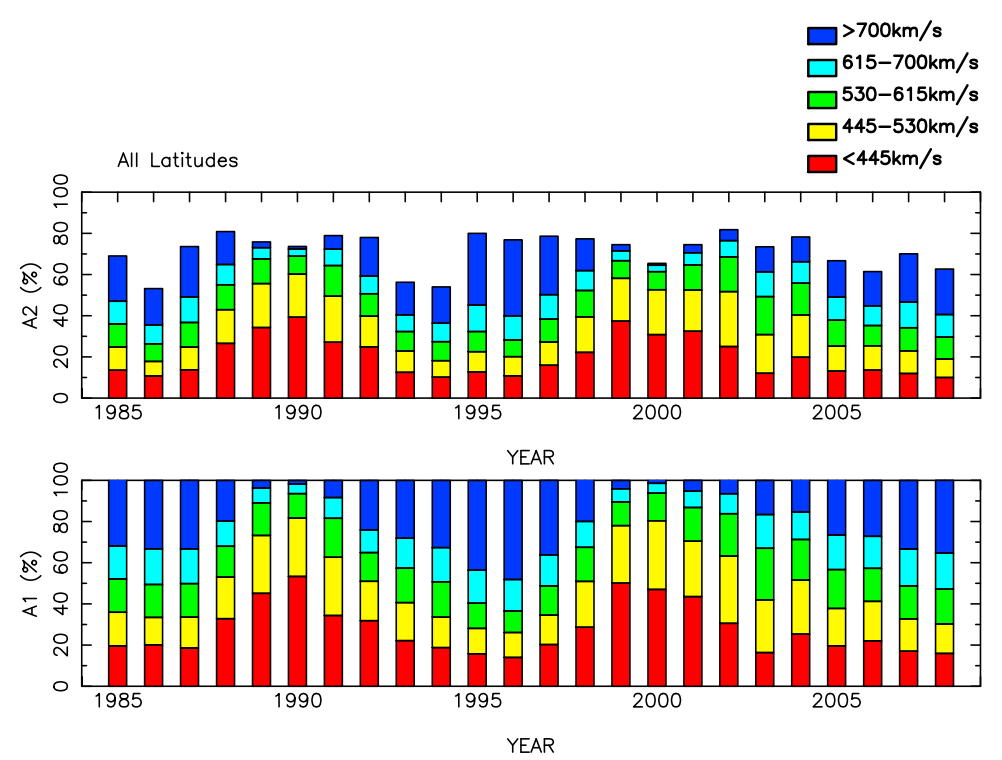
\includegraphics[width=0.8\textwidth]{fig_theory/sw_speed_distribution.PNG}
            \caption{Changes is the fractional areas divided by solar wind speed from 1985 to 2008. On the top, fractional areas compared to the whole surface of the Sun are visible, while on the bottom, fractional areas compared to the measured surface area of the Sun are visible. The colour codes are the following: red: $<445\,km/s$; yellow $445-530\,km/s$; green $530-615\,km/s$; cyan: $615-700\,km/s$; blue: $>700\,km/s$. Source: \cite{2010tokumaru}}
            \label{fig:sw_speeds}
        \end{figure}\\
        To observe and understand the different properties of solar wind and the Interplanetary Magnetic Field during different solar activity levels, the data used in this report (more in Section \ref{sec:data}) has been split into 3 categories, based in the solar activity level: minimum solar activity, intermediate solar activity and maximum solar activity. This process required a data set containing the minimum, intermediate and maximum periods, with their start and finish date. For this, data from the SILSO database (\textit{SILSO data/image, Royal Observatory of Belgium, Brussels}) has been used.\\ \\
        The cycles have been split, so that any time period between a minimum and a maximum (and vice versa) have been split into 3 time period with equal length: the third closest to the minimum would be considered to be minimum solar activity, the third closest to the maximum would be considered to be maximum solar activity and the third between these would be considered to be intermediate solar activity. Then, a list of these activity periods was created, including the activity level, the start date and the end date. The method described before means that from 1 full solar cycle, 6 separate activity periods have been created: 2 minimum solar activity periods, 2 intermediate solar activity periods and 2 maximum solar activity periods.
    \subsection{Equipment}\label{sec:equipment}
        The data used in this report has been collected by the MAG and the SWEPAM instruments on the NASA's Advanced Composition Explorer (ACE)\cite{1998ace}. ACE is currently on a close orbit around Lagrange Point 1 (L1). The position of L1 Point and hence the position of ACE is shown on Figure \ref{fig:l1}, marked L1.\\
        \begin{figure}[t!]
            \centering
            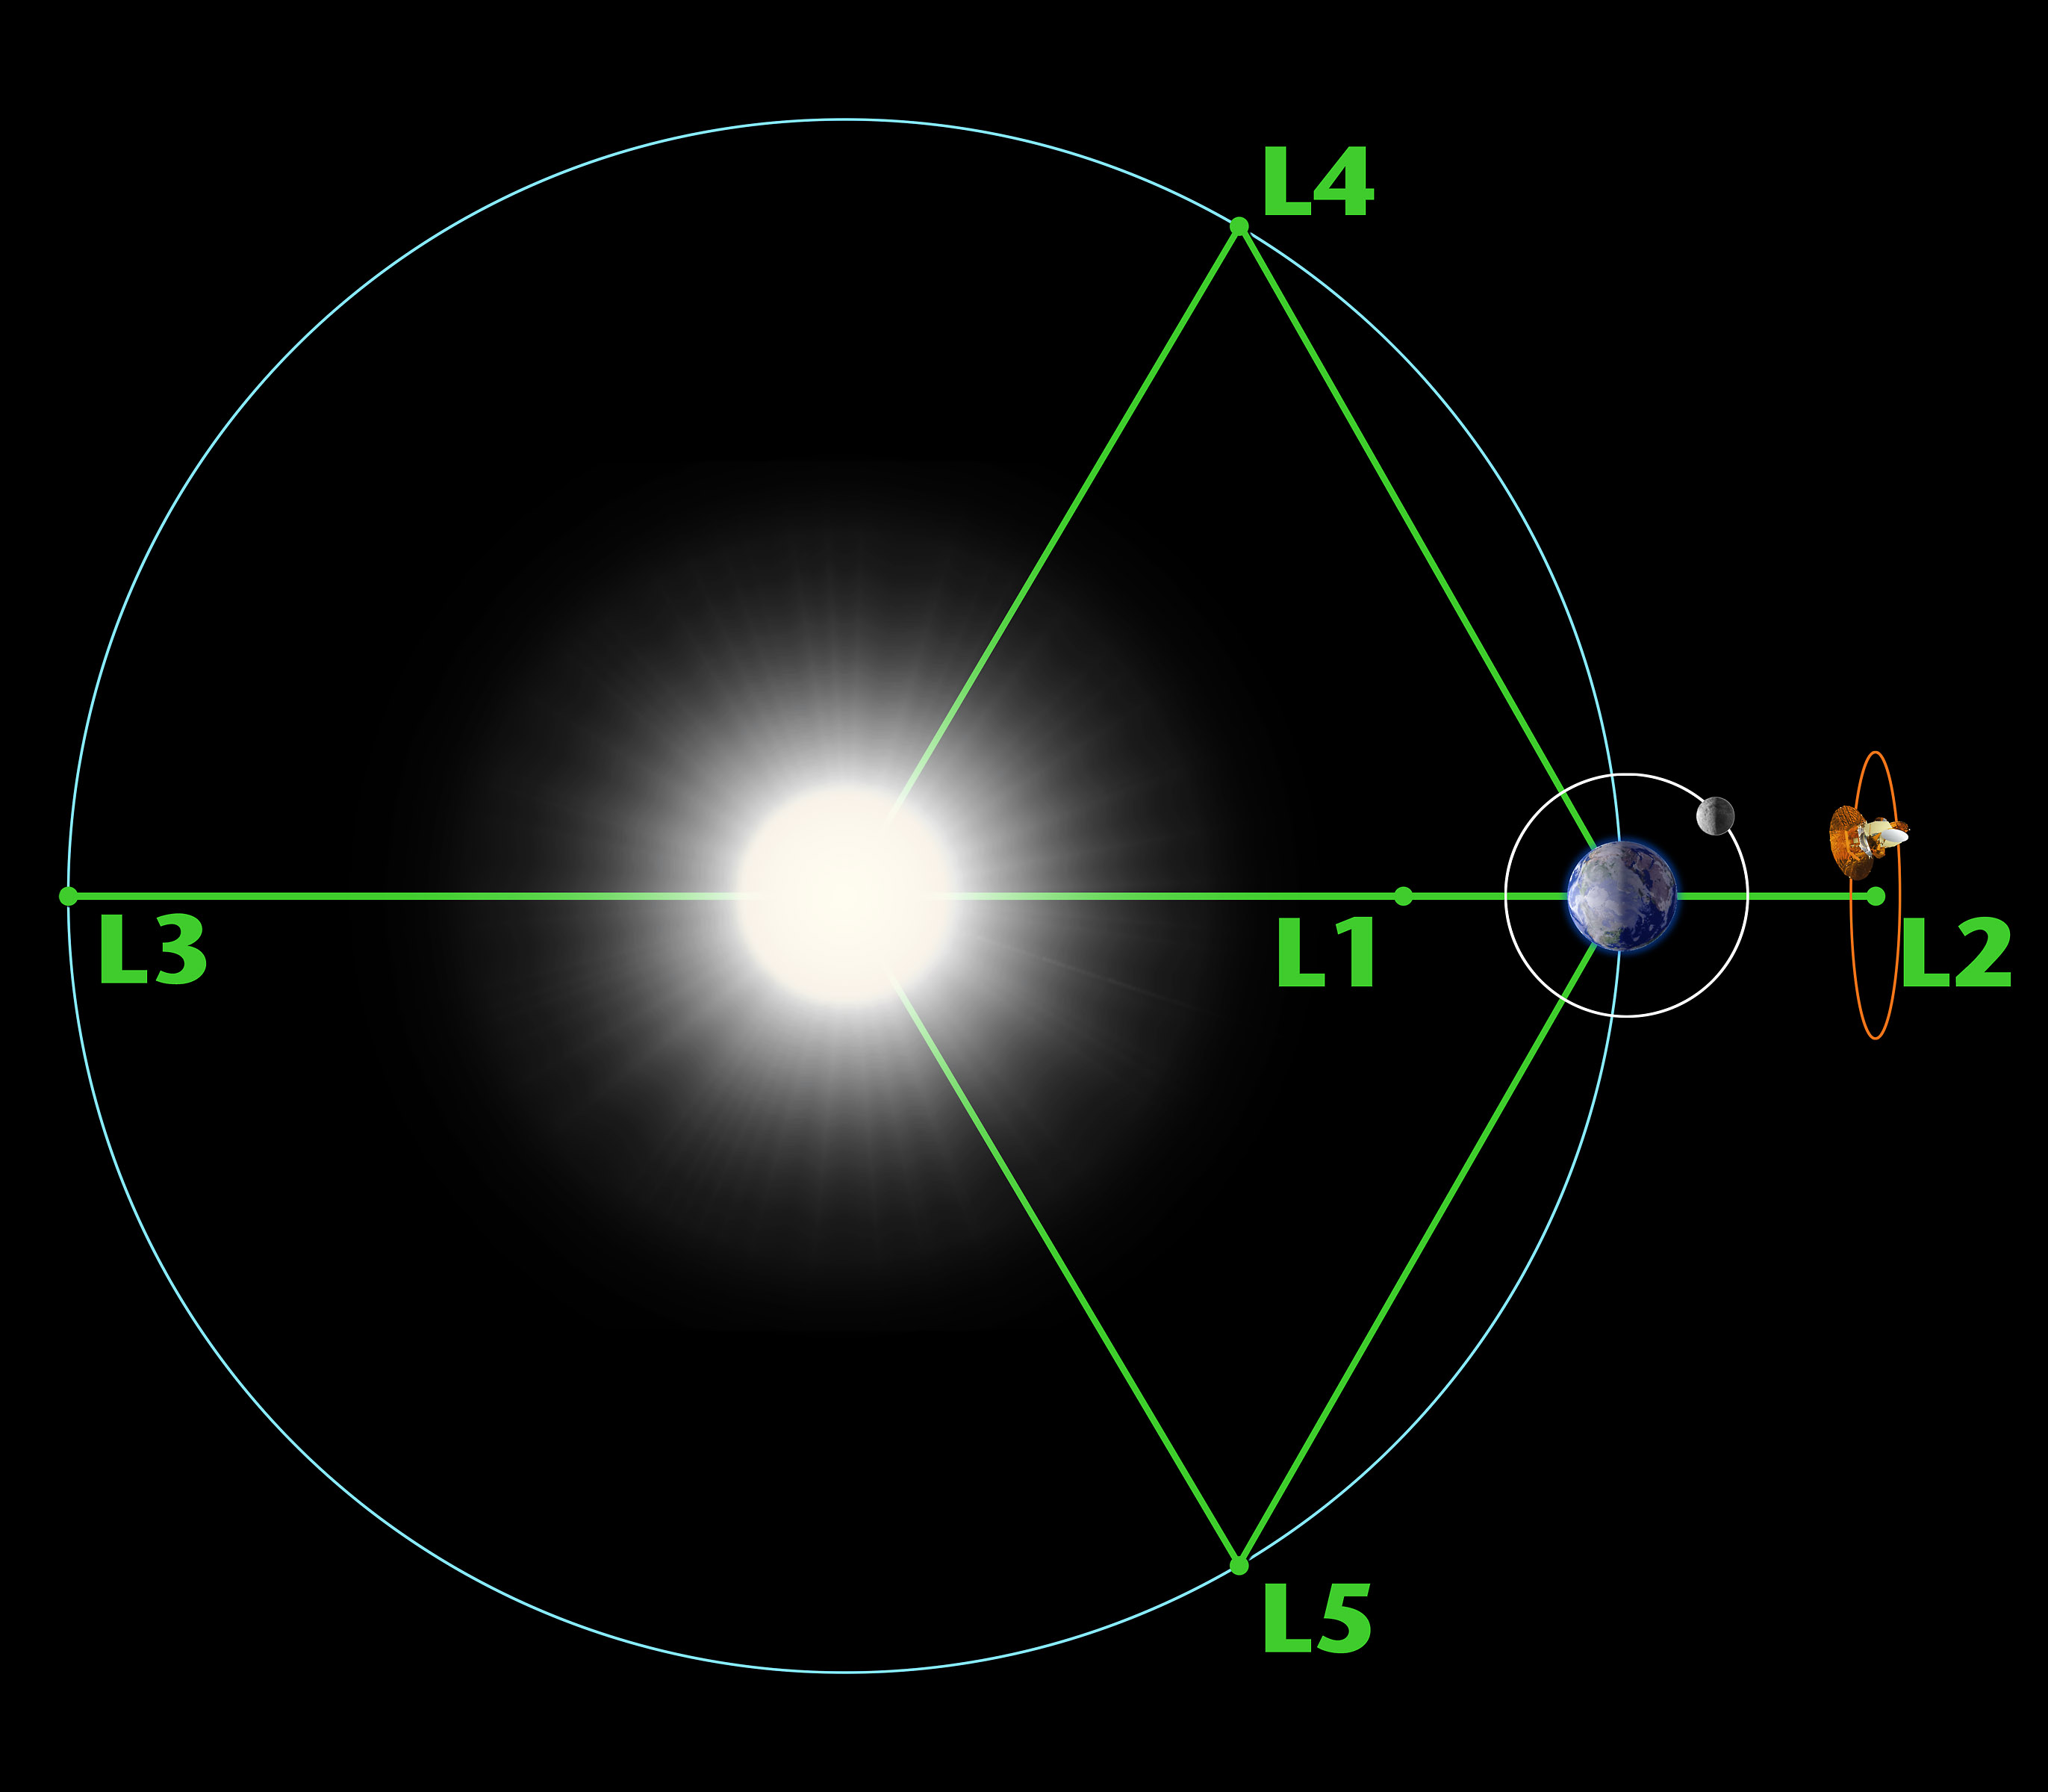
\includegraphics[width=0.6\textwidth]{fig_theory/lagrange.jpg}
            \caption{Positions of Lagrange Points. Lagrange Points are points in space, at which small-mass objects will stay in place, when compared to two certain large-mass objects (e.g. the Sun and the Earth). The ACE can be found orbiting the L1 Point, as it's a great place to measure the properties of the solar wind without having to correct the orbit of the satellite. Figure not to scale. Source: \cite{lagrangeimage}}
            \label{fig:l1}
        \end{figure}\\
        Measurements of the Interplanetary Magnetic Field have been collected using the magnetometer on the ACE\cite{1998acemag}. Measurements of the solar wind velocity have been collected using the Solar Wind Electron Proton Alpha Monitor on the ACE\cite{1998aceswepam}. The raw data has been retrieved from \hlink{https://cdaweb.gsfc.nasa.gov/}
    \subsection{Generalised Extreme Value Distribution}\label{sec:gev}
        The Generalised Extreme Value Distribution is used to model the extreme value of data sets and to extrapolate even more extreme values, using an existing data set. It can model both extremely high or extremely low data, depending on the context. For example modelling extremely high data would be the sea-level in a port. Modelling extremely low data would be the solar wind velocity between the Sun and the Earth, using the GSM coordinate system (due to the coordinate system, the more negative values would be interpreted as more extreme). Multiple different methods and distributions exists to model the extreme values of a data set.\\ \\
        The Generalised Extreme Value Distribution uses the maximum (or minimum) values from several periods of the same length from the same data set (e.g. the maximum value each day). The maximum value from each period is represented by $M_n$:
        \begin{equation}
            M_n = max\{X_1, X_2, ..., X_{n-1}, X_n\}
        \end{equation}
        where $n$ represents the period it's been taken from (e.g. the day the measurement was taken, is one's using daily maxima) and $X_n$ is the nth variable in the given period.\\
        When $n\rightarrow \infty$:
        \begin{equation}
            Pr\Bigg\{ \frac{M_n - b_n}{a_n} \leq z\Bigg\} \rightarrow G(z)
        \end{equation}
        where $G(z)$ is the Generalised Extreme Value Distribution\cite{2001coles}.\\ \\
        The cumulative distribution function for the Generalised Extreme Value Distribution is represented by the following equation\cite{2001coles}:
        \begin{equation}
            G(z) = exp\Bigg [-\Bigg [1+\xi \Bigg (\frac{z-\mu}{\sigma}\Bigg )\Bigg ]^{-1/\xi}\Bigg ]
        \end{equation}
        where $\xi$ is the shape parameter, $\mu$ is the location parameter and $\sigma$ is the scale parameter. If $\xi=0$, the equation above changes to the equation below:
        \begin{equation}
            G(z) = exp\Bigg [exp\Bigg [\Bigg (-\frac{z-\mu}{\sigma}\Bigg )\Bigg ]\Bigg ]
        \end{equation}\\
        Figure \ref{fig:gev} shows the cumulative distribution function and the probability density function of GEV, with varying parameters.\\
        \begin{figure}[t!]
            \centering
            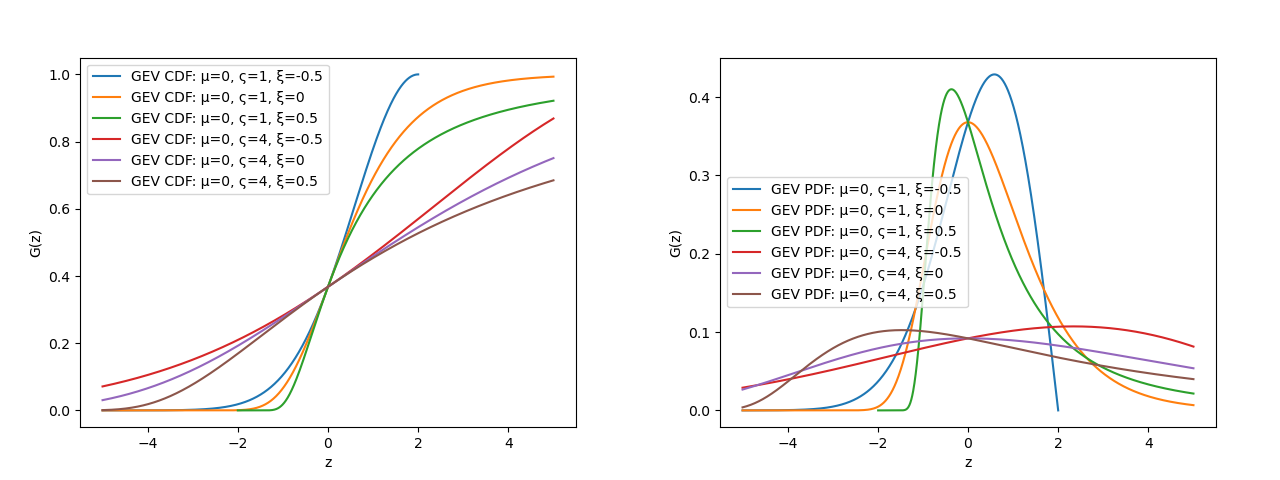
\includegraphics[width=\textwidth]{fig_theory/gev.png}
            \caption{Cumulative distribution functions (left) and probability density functions (right) for the Generalised Extreme Value Distribution, with constant $\mu$ (location) parameter and varying $\sigma$ (scale) and $\xi$ (shape) parameters.}
            \label{fig:gev}
        \end{figure}\\
        To model the distribution of minima, $-z$ should be used instead of $z$. The parameters of the distribution can be determined using several methods (e.g. using maximum likelihood estimation).
    \subsection{Return Levels for Extreme Value Distributions}\label{sec:returnlevel}
        The return level ($z_p$) represents the value expected to be exceeded exactly once during a set period, called the return period ($r$) or conversely, the return period of a value is the period during which the value will be exceeded exactly once.
        The return level can be calculated using the following formula\cite{2001coles}:
        \begin{equation}
            z_p = \mu-\frac{\sigma}{\xi}\Bigg( 1-\Bigg( -ln\Bigg( 1-\frac{1}{r}\Bigg) \Bigg) ^{-\xi}\Bigg)  
        \end{equation}
        where $z_p$ is the return level (or if minima values were used, $-z_p$ is the return level), $\xi$ is the shape parameter, $\mu$ is the location parameter and $\sigma$ is the scale parameter.\\ \\
        To calculate the errors in the return level, one needs to calculate the observed information matrix ($I_E(\xi,\mu,\sigma)$), then use it to calculate the variance-covariance matrix (V):
        \begin{equation}
            I_E(\xi,\mu,\sigma) = 
            \begin{bmatrix}
                    -\frac{\partial ^2l}{\partial \xi^2} & -\frac{\partial ^2l}{\partial \xi \partial \mu} & -\frac{\partial ^2l}{\partial \xi \partial \sigma} \\
                    -\frac{\partial ^2l}{\partial \mu \partial \xi} & -\frac{\partial ^2l}{\partial \mu^2} & -\frac{\partial ^2l}{\partial \mu \partial \sigma} \\
                    -\frac{\partial ^2l}{\partial \sigma \partial \xi} & -\frac{\partial ^2l}{\partial \sigma \partial \mu} & -\frac{\partial ^2l}{\partial \sigma^2}
            \end{bmatrix}
        \end{equation}
        and
        \begin{equation}
            V=I_E^{-1}(\xi,\mu,\sigma)
        \end{equation}
        Using the variance-covariance matrix, the values for the standard error in each parameter can be retrieved, using:
        \begin{equation}
            V=
            \begin{bmatrix}
                    SE_\xi^2 & \ldots & \ldots \\
                    \ldots & SE_\mu^2 & \ldots \\
                    \ldots & \ldots & SE_\sigma^2
            \end{bmatrix}
        \end{equation}
        The variance of the return level then can be calculated using the following formula:
        \begin{equation}
            Var(\hat z_p)\approx \Delta z_p^TV\Delta z_p
        \end{equation}
        where
        \begin{equation}
            \Delta z_p^T=\Bigg [\frac{\partial z_p}{\partial \xi}, \frac{\partial z_p}{\partial \mu}, \frac{\partial z_p}{\partial \sigma}\Bigg ]
        \end{equation}
\section{Method and Data Processing}\label{sec:method}
    \subsection{The Data}\label{sec:data}
        As already mentioned in Section \ref{sec:equipment}, the data used in this report has been collected by the MAG\cite{1998acemag} and the SWEPAM\cite{1998aceswepam} instruments on the NASA's Advanced Composition Explorer (ACE)\cite{1998ace}. The data collected by the MAG instrument (from now on, MAG data), used to analyse the Interplanetary Magnetic Field at L1 ranges from 01/01/1998 to 25/07/2021, while the data collected by the SWEPAM instrument (from now on, SWEPAM data), used to analyze the solar wind speed at L1 ranges from 04/02/1998 to 17/01/2021, meaning that for both data sets, more than 22 years of data has been used. To determine the solar wind ram pressure, data points only found in both of these data sets have been used, therefore the solar wind ram pressure data ranges from 04/02/1998 to 17/01/2021. Both data sets include the data divided in to separate files day by day and include measurements of the strength of the Interplanetary Magnetic Field (MAG data) and the solar wind speed (SWEPAM data) in form of 3-dimensional vectors, representing the data in GSM coordinates. Throughout this report, it should be assumed that data concerning the strength of the Interplanetary Magnetic Field is in units of nT, data concerning the solar wind speed is in units of km/s and data concerning the solar wind ram pressure is in units of nPa.\\ \\
        It is important to note, that while the MAG data includes measurements every second (86400 measurements per day), and hence it can be assumed, that the difference between the measured daily maxima (minima) and the actual daily maxima (minima) is negligible, the same cannot be stated about the SWEPAM data. The SWEPAM data includes measurements every hour (24 per measurements day), therefore a slight difference between the measured daily maxima (minima) and the actual daily maxima (minima) should be expected and the result should be used with caution.\\ \\
        As already mentioned in Section \ref{sec:solarcycle}, data concerning the solar activity periods (more accurately, solar activity maximums and minimums) have been found in the SILSO database (\textit{SILSO data/image, Royal Observatory of Belgium, Brussels}).
    \subsection{Assumptions and Data Processing}\label{sec:dataproc}
        Several assumptions have been made when processing the data and applying distribution functions. These assumptions have been made about the data itself and the behaviour of the solar wind as well:
        \begin{itemize}
            \item It has been assumed, that the data points within each period (from which the maxima and the minima have been selected), the data points would behave like random samples of an arbitrary distribution, and therefore would be independent. This is not entirely true, as the data about the IMF strength and the solar wind speed is driven by several factors, like solar activity, the previous measurements and the state of the IMF (in case of the solar wind speed) or the state of the solar wind (in case of the IMF strength). As solar wind speed and the IMF strength are related due to Alfvén's Theorem\cite{1976alfven}, they depend on each other. In Section \ref{sec:dailydist}, the distributions fitted on the data points show, that this is mostly negligible, due to the large amount of data available.
            \item It has been assumed, that solar wind only consists of electrons and protons. This is relevant, when determining the solar wind ram pressure, as this assumption means heavier ions have not been taken into account when determining the mean mass of solar wind particles. As the abundance of heavier ions in solar wind is small (approximately 5\%\cite{2006schwenn}), this assumption appears to be justifiable.
            \item It has been assumed, that the actual maximum (minimum) value of each day is the largest (smallest) measured value. This assumption has been made due to availability of data.
            \item The solar activity levels have been assumed to have the same time-span from a solar activity minimum to a solar activity maximum (and from a solar activity maximum to a solar activity minimum). This means, that the periods between solar activity minimums and solar activity maximums have been divided to a period of minimum solar activity, intermediate solar activity and maximum solar activity, all of which are the same length. This assumption was made due to a lack of a better method to separate these solar activity levels.
        \end{itemize}\\
        The data processing method to obtain the exact distributions for the Interplanetary Magnetic Field strengths and for the solar wind speeds are almost identical. The method below has been used to produce the distribution graphs in Section \ref{sec:dailydist} (except for the solar wind ram pressure distributions).
        \begin{enumerate}
            \item A list of solar activity periods have been prepared, containing the dates the periods begin and end, and the type of period it is (minimum, intermediate or maximum solar activity).
            \item For every file (one day of measurements), the following process has been followed: the invalid measurements from the IMF strength (and alike from the solar wind speed) data for x, y and z coordinates have been removed and the daily minima and maxima have been determined. These data points have been separated based on coordinate, solar activity the given day belongs to and whether the list contains the minima or the maxima for the given solar activity and coordinate.\label{stepcontinue}
            \item To each of the data points in a list, the ratio of data points lower (higher for minima) has been assigned. For each property (coordinate, solar activity level and minima/maxima), a line of best fit was fitted, using Generalised Extreme Value Distribution and the least square method, then the parameters of the distribution have been determined. Graphs of cumulative distributions functions and probability density functions (based on the parameters determined by the cumulative density functions) have been plotted.
            \item Using the method described in Section \ref{sec:returnlevel}, the errors in the parameters have been determined.
            \item For each property, a graph of return level against return period has been plotted. The return levels have been plotted for return period values between 0.1 year and 1000 years. Then, using the method described in Section \ref{sec:returnlevel}, the errors in the return levels have been determined.
        \end{enumerate}
        The process to plot similar graphs for the solar wind ram pressure includes an additional step. Before determining the maxima and the minima for a period, the following formula has been used to calculate the solar wind ram pressure for every data point in a period:
        \begin{equation}
            P=n*m_p*V^2
        \end{equation}
        where $n$ is the proton density (the electron density is negligible, as electrons have negligible mass and therefore do not contribute to the solar wind ram pressure), $m_p$ is the mass of a proton and $V$ is the solar wind bulk velocity. Then, the daily minima and maxima have been determined and the same process from Step \ref{stepcontinue}. has been followed. It is important to note, that for solar wind ram pressure, the data has not been separated based on coordinates, as solar wind ram pressure in the y and z-directions is negligible due to the small velocity components.
    \subsection{Distributions of the strength of the Interplanetary Magnetic Field and of the solar wind speed}
        Using data described in Section \ref{sec:data}, an array of histograms (Figure \ref{fig:hist_imf}) has been created to show the more extreme values as well.
        \begin{figure}[t!]
            \centering
            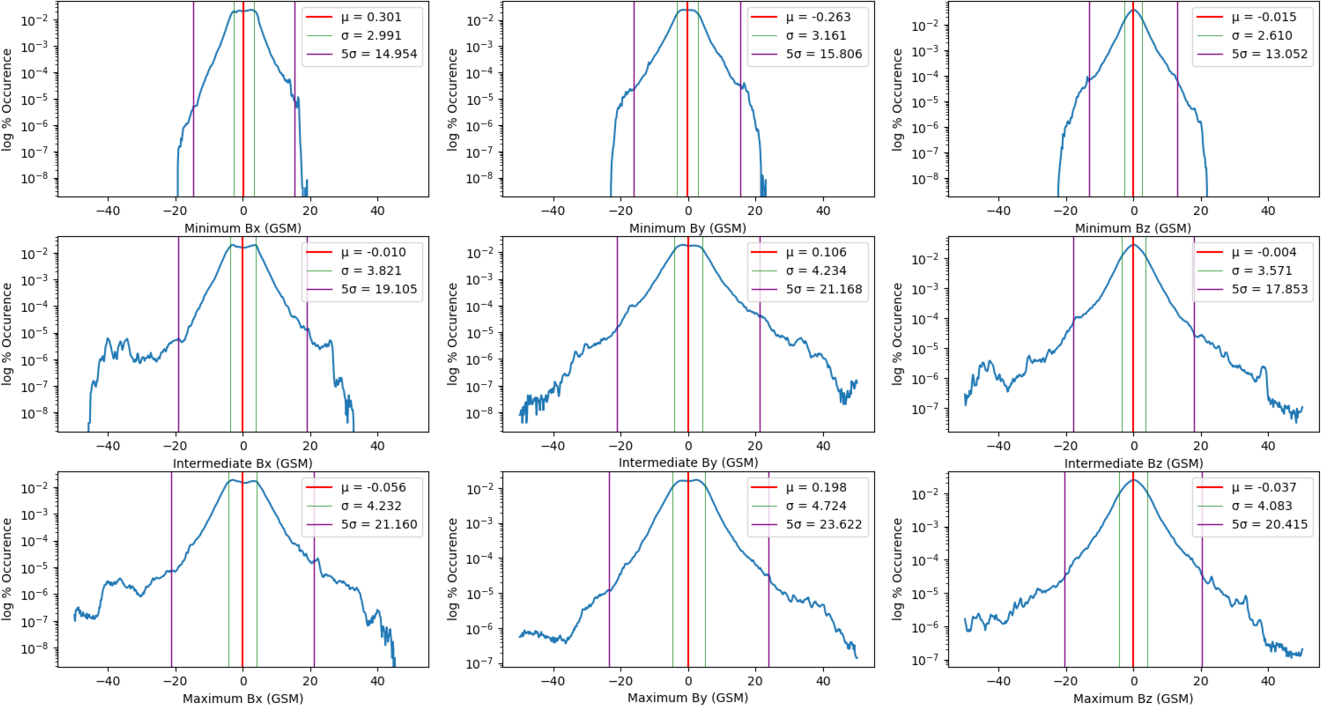
\includegraphics[width=\textwidth]{fig_introduction/hist_imf_strength.png}
            \caption{Histograms showing the strength of the Interplanetary Magnetic Field at Lagrange point L1 (in nT). Data has been separated into 9 different batches based on coordinates in the GSM coordinate system and the solar activity level at the time of measurement. Each row refers to a different solar activity level (minimum, intermediate or maximum) and each column refers to a different coordinate (x, y or z). The red lines indicate the mean, the green lines indicate $1\sigma$ distance from the mean and the purple lines indicate $5\sigma$ distance from the mean.}
            \label{fig:hist_imf}
        \end{figure}
        Comparing Figures \ref{fig:russellBX}, \ref{fig:russellBY} and \ref{fig:russellBZ} (from previous studies) to Figure \ref{fig:hist_imf}, two important points can be made:
        \begin{itemize}
            \item The middle parts (between approximately $4\sigma -5\sigma$) of the graphs on Figure \ref{fig:hist_imf} almost exactly match the graphs on Figures \ref{fig:russellBX}, \ref{fig:russellBY} and \ref{fig:russellBZ}. This means that even when using slightly different data, anyone could arrive to the same solutions and conclusions.
            \item The end tails on Figure \ref{fig:hist_imf} are not visible on Figures \ref{fig:russellBX}, \ref{fig:russellBY} and \ref{fig:russellBZ}, therefore Figure \ref{fig:hist_imf} is more useful when examining the unusual behaviour of the Interplanetary Magnetic Field outside the zone of influence of Earth's magnetic field.
        \end{itemize}
        Examining Figure \ref{fig:hist_imf}, the quick drop-off at around -20nT on the top row of graphs shows that we can expect no extremely low or extremely high value for magnetic field measurements at the L1 point. More extreme values appear on the graphs of intermediate and maximum solar activity for $B_y$ and $B_z$, but they mostly seem to drop off at a fairly constants rate, suggesting that this is not due to an external effect. This does not seem to hold for the graphs showing the intermediate and maximum solar activity for $B_x$. The end tails in these graphs do not drop off smoothly, but instead have quite a few spikes between -30nT and -40 nT. This suggest that the ordinary behaviour of the IMF breaks, most likely due to an external event, like a coronal mass ejection, which would release a large amount of fast solar wind, carrying a larger magnetic field due to Alfvén's theorem\cite{1976alfven}.\\
        \begin{figure}[t!]
            \centering
            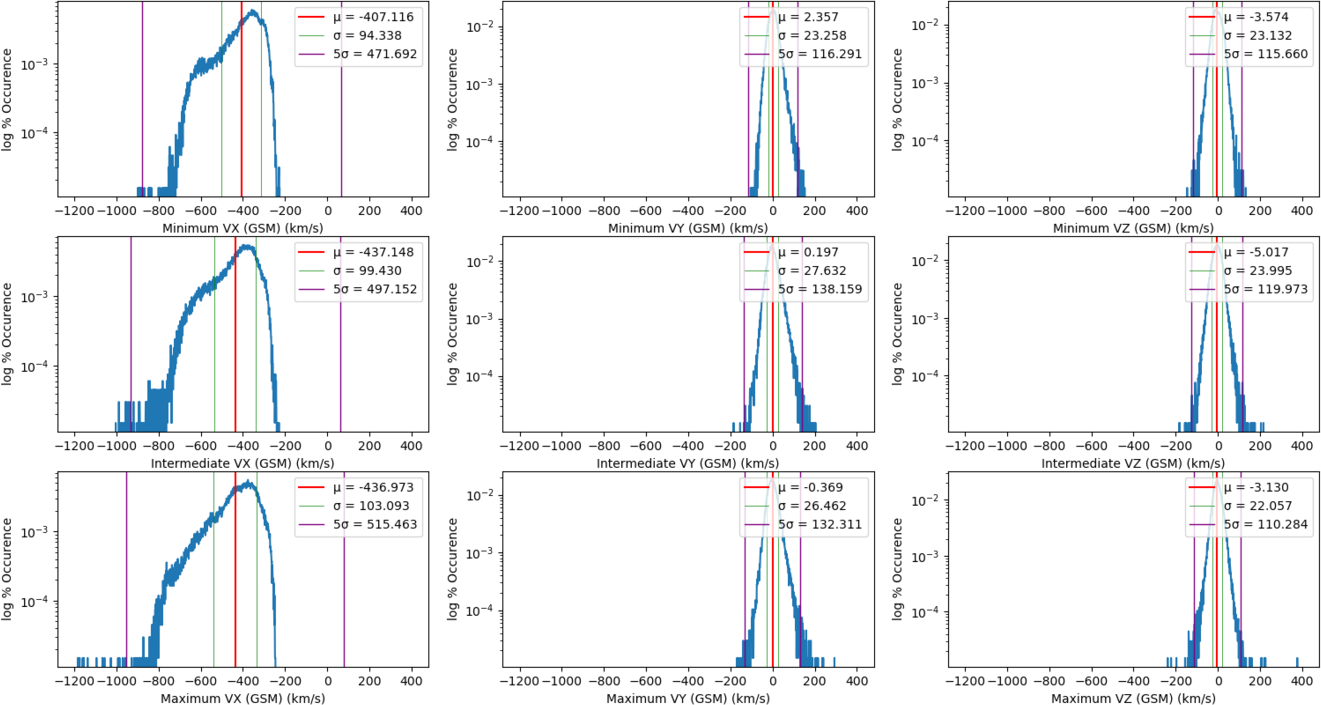
\includegraphics[width=\textwidth]{fig_theory/hist_sw_velocity.png}
            \caption{Histograms showing the velocity of the solar wind at point L1 (in km/s). Data has been separated into 9 different batches based on coordinates in the GSM coordinate system and the solar activity level at the time of measurement. Each row refers to a different solar activity level (minimum, intermediate or maximum) and each column refers to a different coordinate (x, y or z). The red lines indicate the mean, the green lines indicate $1\sigma$ distance from the mean and the purple lines indicate $5\sigma$ distance from the mean.}
            \label{fig:hist_sw}
        \end{figure}\\
        Figure \ref{fig:hist_sw} shows the distribution of solar wind speed separated based on solar activity level. The most interesting graphs are the histograms of the distribution of $V_x$. $V_y$ and $V_z$ have a fairly even distribution centered around $0\,$km/s with a low variance, no matter the solar activity level. The $B_x$ histograms show a sudden drop at around $-250\,$km/s, suggesting that solar wind is rarely slower than that. The most common velocity on these graphs is around $-400\,$km/s, which matches the average velocity of slow solar wind\cite{2001russell} (more in Section \ref{sec:solarwind}). A small spike is visible at around $-700\,$km/s, which approximately matches the average velocity of fast solar wind\cite{2001russell}. This suggests that slow solar wind is much more abundant, than fast solar wind.
    \subsection{Distributions of Daily Minima and Maxima}\label{sec:dailydist}
        \begin{figure}[t!]
            \begin{minipage}{0.48\textwidth}
                \centering
                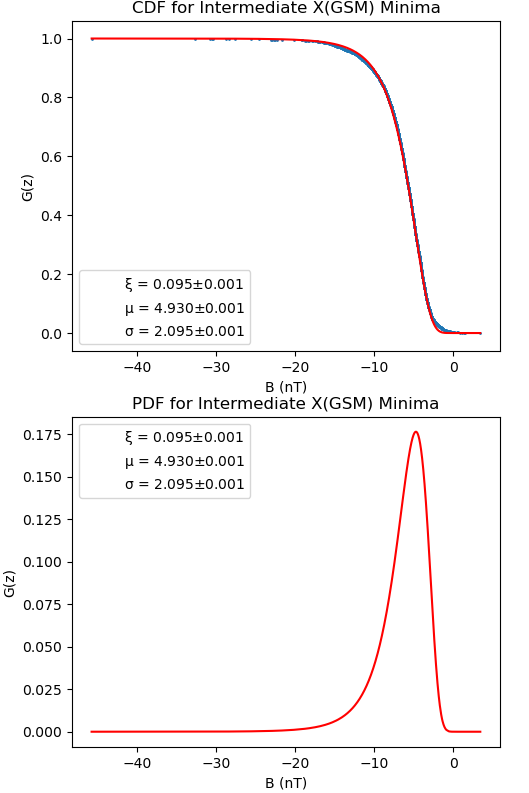
\includegraphics[width=\textwidth]{fig_method/MFIintXmin.png}
                \caption{Cumulative distribution function (top) and probability density function (bottom) of the daily minima of the IMF strength in the x-direction, during intermediate solar activity.}
                \label{fig:MFIintXmin}
            \end{minipage}
            \hfill
            \begin{minipage}{0.48\textwidth}
                \centering
                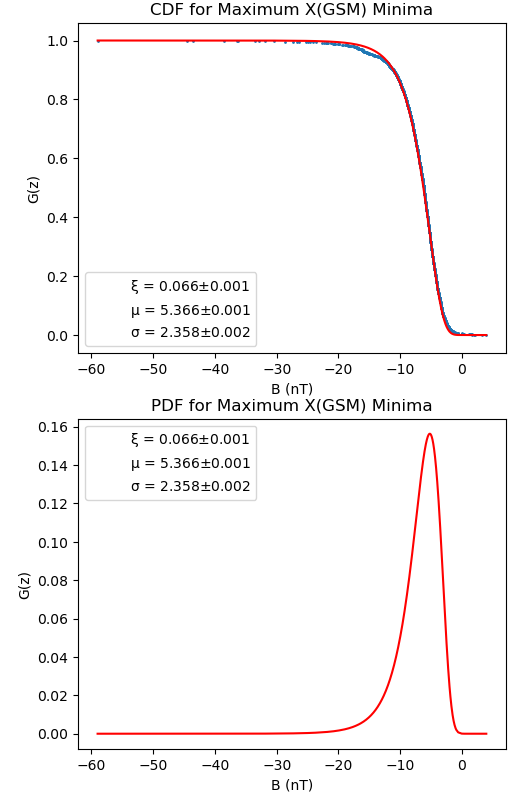
\includegraphics[width=\textwidth]{fig_method/MFImaxXmin.png}
                \caption{Cumulative distribution function (top) and probability density function (bottom) of the daily minima of the IMF strength in the x-direction, during maximum solar activity.}
                \label{fig:MFImaxXmin}
            \end{minipage}
        \end{figure}
        \begin{figure}[t!]
            \begin{minipage}{0.48\textwidth}
                \centering
                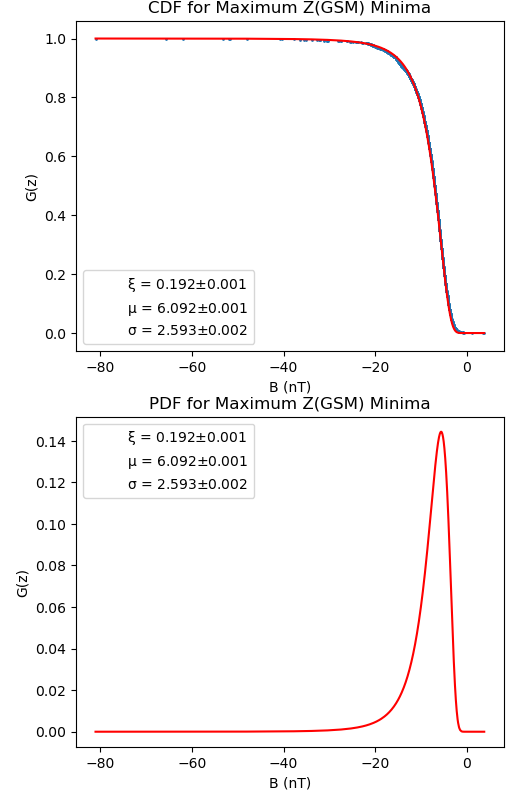
\includegraphics[width=\textwidth]{fig_method/MFImaxZmin.png}
                \caption{Cumulative distribution function (top) and probability density function (bottom) of the daily minima of the IMF strength in the y-direction, during maximum solar activity.}
                \label{fig:MFImaxZmin}
            \end{minipage}
            \hfill
            \begin{minipage}{0.48\textwidth}
                \centering
                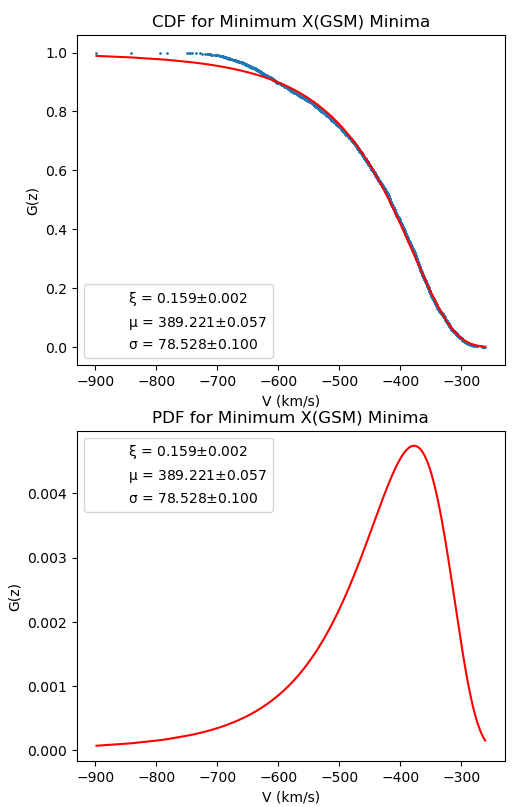
\includegraphics[width=\textwidth]{fig_method/SWEminXmin.png}
                \caption{Cumulative distribution function (top) and probability density function (bottom) of the daily minima of the solar wind speed in the x-direction, during minimum solar activity.}
                \label{fig:SWEminXmin}
            \end{minipage}
        \end{figure}
        \begin{figure}[t!]
            \begin{minipage}{0.48\textwidth}
                \centering
                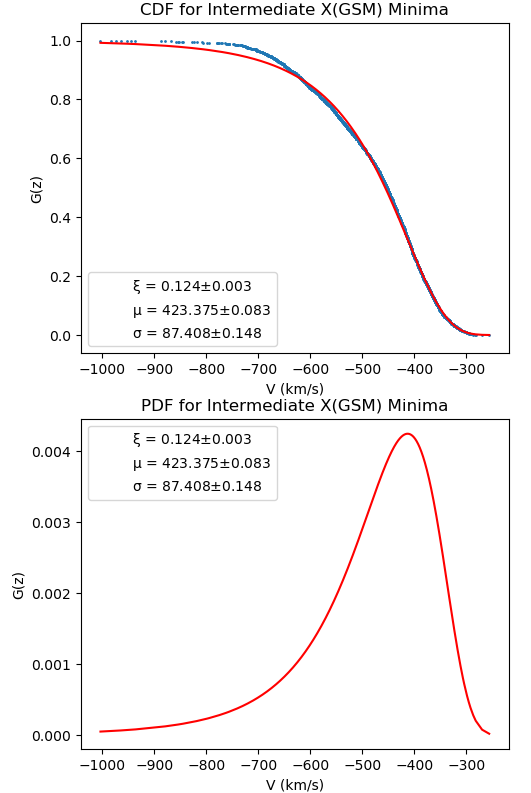
\includegraphics[width=\textwidth]{fig_method/SWEintXmin.png}
                \caption{Cumulative distribution function (top) and probability density function (bottom) of the daily minima of the solar wind speed in the x-direction, during intermediate solar activity.}
                \label{fig:SWEintXmin}
            \end{minipage}
            \hfill
            \begin{minipage}{0.48\textwidth}
                \centering
                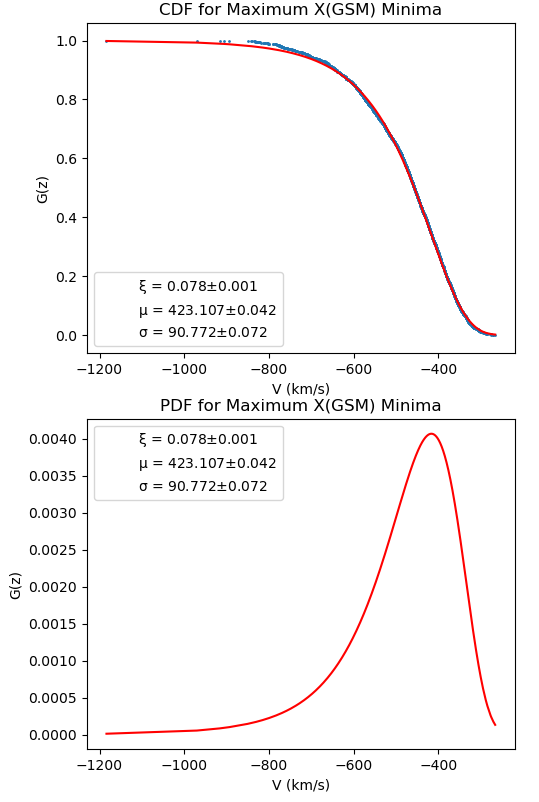
\includegraphics[width=\textwidth]{fig_method/SWEmaxXmin.png}
                \caption{Cumulative distribution function (top) and probability density function (bottom) of the daily minima of the solar wind speed in the x-direction, during maximum solar activity.}
                \label{fig:SWEmaxXmin}
            \end{minipage}
        \end{figure}
        After following the procedure described in Section \ref{sec:dataproc}, two graphs for each combination of the three solar activity levels (minimum, intermediate and maximum), coordinate (x, y and z) and daily minima or maxima has been produced: a graph of the cumulative distribution function and a graph of the probability density function. This section aims to describe the and point out the most important properties of these graphs, that are relevant to the topic of the report. The effects on the return levels/return periods of the differences in the parameters describing comparable graphs is hard to predict from these graphs, and therefore these comparisons will mainly be discussed in Section \ref{sec:gev}. The parameters of the distributions in this section and Section \ref{sec:returnperiod} can be found in Table \ref{tab:parameters}.\\
        \begin{table}[t!]
            \begin{center}
                \begin{tabular}{|l|c|c|c|} \hline
                    \textit{Distribution}&$\xi$&$\mu$&$\sigma$\\ \hline
                    IMF Intermediate X Minima&0.095\pm 0.001&4.930\pm 0.001&2.095\pm 0.001\\ \hline
                    IMF Maximum X Minima&0.066\pm 0.001&5.366\pm 0.001&2.358\pm0.002\\ \hline
                    IMF Maximum Z Minima&0.192\pm 0.001&6.092\pm 0.001&2.593\pm 0.002\\ \hline
                    SWS Minimum X Minima&0.159\pm 0.002&389.221\pm 0.057&78.528\pm 0.100\\ \hline
                    SWS Intermediate X Minima&0.124\pm 0.003&423.375\pm 0.083&87.408\pm 0.148\\ \hline
                    SWS Maximum X Minima&0.078\pm 0.001&423.107\pm0.042&90.772\pm 0.072\\ \hline
                    P Intermediate Maxima&0.430\pm 0.001&20.402\pm0.005&11.560\pm 0.008\\ \hline
                    P Maximum Maxima&0.399\pm 0.001&19.655\pm 0.003&12.840\pm 0.006\\ \hline
                \end{tabular}
                \caption{The parameters of the distributions described in Section \ref{sec:dailydist} and the equations describing the return periods and return levels in Section \ref{sec:returnperiod}. Using the equations in these sections and substituting the parameters, the distributions and relationship in these sections can be reconstructed. IMF refers to the Interplanetary Magnetic Field, SWS refers to the solar wind speed and P refers to the solar wind ram pressure. Minimum, Intermediate and Maximum refers to the solar activity level, while X or Z refers to the coordinates and Minima/Maxima refers to whether the distribution described daily minima or maxima. \label{tab:parameters}}
            \end{center}
        \end{table}\\
        The graphs on Figures \ref{fig:MFIintXmin} and \ref{fig:MFImaxXmin} describe the distributions of the daily minima of the IMF in the x-direction, during intermediate and maximum solar activity, respectively. The parameters acquired for these graphs (and the fact that they are somewhat similar) suggest that the IMF acts in similar ways during intermediate and maximum solar activity. The small differences between these parameters will mean some difference between the expected return level for a given return period (more in Section \ref{sec:returnperiod}). Studying these distributions is important, as the strength of the IMF in the x-direction often gives good indications of the strength of the solar wind heading towards Earth.\\ \\
        The graphs on Figure \ref{fig:MFImaxZmin} describe the distribution of the daily minima of the IMF in the z-direction, during maximum solar activity. For the purposes of this study, daily maxima could have been selected as well, as the distribution of the magnetic field strength in the z-direction is fairly symmetric around $B_z=0\,$nT (see Figure \ref{fig:hist_imf}). The graph of daily minima has been selected, as this will give an easier way to predict the return period of a `Carrington Event'-like geomagnetic storm (more in Section \ref{sec:carrington}).\\ \\
        The graphs on Figures \ref{fig:SWEminXmin}, \ref{fig:SWEintXmin} and \ref{fig:SWEmaxXmin} describe the distributions of the daily minima of the solar wind speed in the x-direction, during minimum, intermediate and maximum solar activity, respectively. While the parameters on Figures \ref{fig:SWEintXmin} and \ref{fig:SWEmaxXmin} are similar mostly similar (except for the shape parameter, $\xi$), the parameters on Figure \ref{fig:SWEminXmin} are more different (smaller location parameter, $\mu$ and smaller scale parameter, $\sigma$), suggesting that the behaviour of the solar wind speed is similar during intermediate and maximum solar activity, while it's different during minimum solar activity. The smaller location parameter would suggest more extreme behaviour during minimum solar activity, while the smaller shape parameter would suggest less extreme behaviour in this period. The overall effects of these parameters will be shown in Section \ref{sec:returnperiod}.\\ \\
        Figures \ref{fig:SWEminXmin} and \ref{fig:SWEintXmin} show a slight digression of the daily minima at around $-800\,$km/s. This is due to the presence of fast solar wind and its large difference of speed from the speed of slow solar wind. This disturbs the otherwise reasonable for of the Generalised Extreme Value Distribution, which would lead to inaccurate return levels and return periods.\\
        \begin{figure}[t!]
            \begin{minipage}{0.48\textwidth}
                \centering
                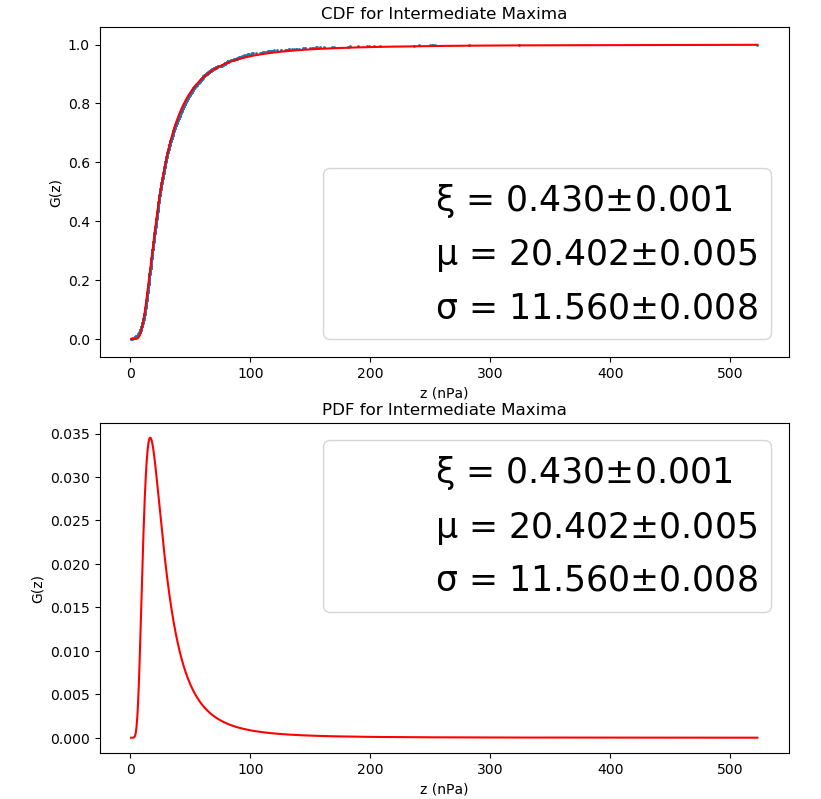
\includegraphics[width=\textwidth]{fig_method/Pintmax.png}
                \caption{Cumulative distribution function (top) and probability density function (bottom) of the daily maxima of the solar wind ram pressure, during intermediate solar activity.}
                \label{fig:Pintmax}
            \end{minipage}
            \hfill
            \begin{minipage}{0.48\textwidth}
                \centering
                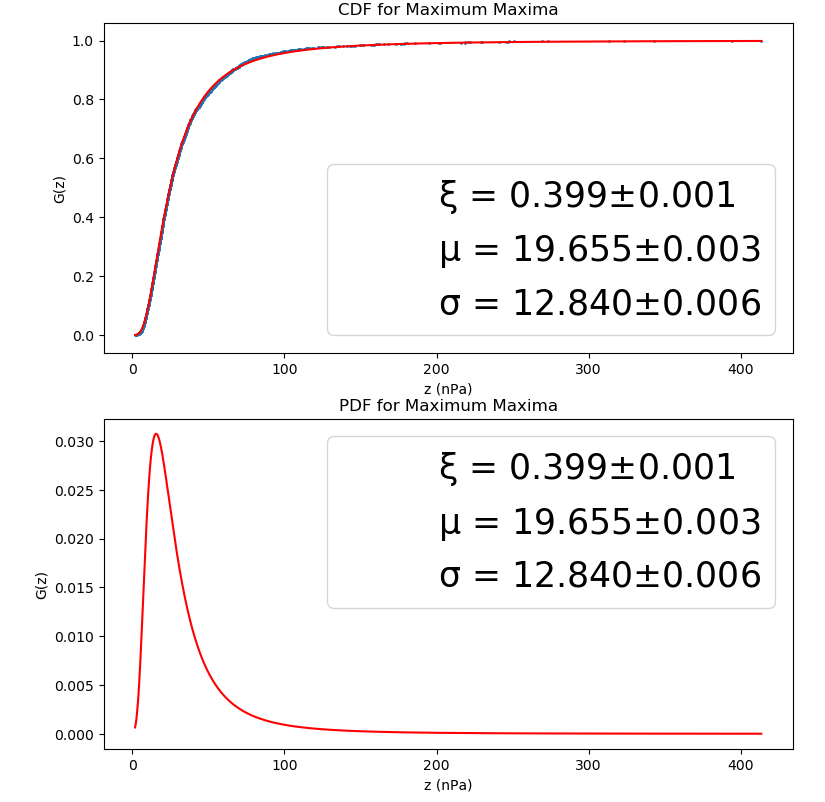
\includegraphics[width=\textwidth]{fig_method/Pmaxmax.png}
                \caption{Cumulative distribution function (top) and probability density function (bottom) of the daily maxima of the solar wind ram pressure, during maximum solar activity.}
                \label{fig:Pmaxmax}
            \end{minipage}
        \end{figure}\\
        The graphs on Figures \ref{fig:Pintmax} and \ref{fig:Pmaxmax} describe the distributions of the daily maxima of the solar wind ram pressure, during intermediate and maximum solar activity, respectively. There is a slight difference between the two graphs in all three parameters, therefore it is incredibly difficult to predict how their return levels for a given return period will relate, before seeing the return level against return period graphs (in Section \ref{sec:returnperiod}).
    \subsection{Return Levels of Daily Minima and Maxima}\label{sec:returnperiod}
        \begin{figure}[t!]
            \begin{minipage}{0.48\textwidth}
                \centering
                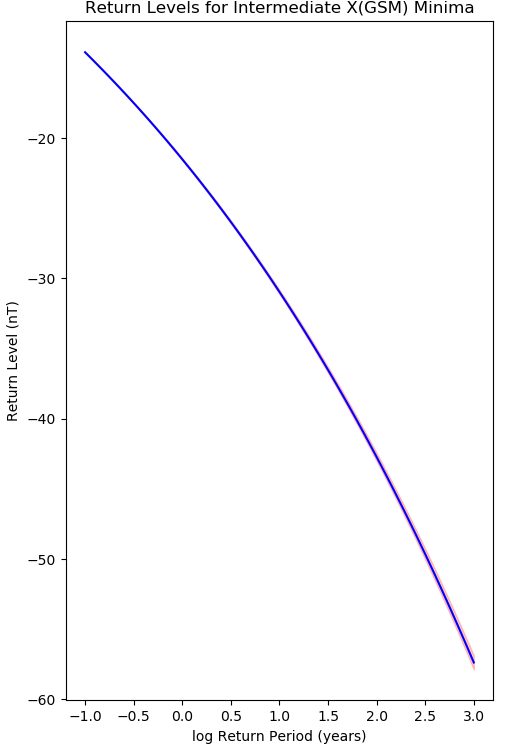
\includegraphics[width=\textwidth]{fig_method/MFIintXminReturn.png}
                \caption{Return Level against $log_{10}$ Return Period graph of the IMF strength in the x-direction, during intermediate solar activity.}
                \label{fig:MFIintXminReturn}
            \end{minipage}
            \hfill
            \begin{minipage}{0.48\textwidth}
                \centering
                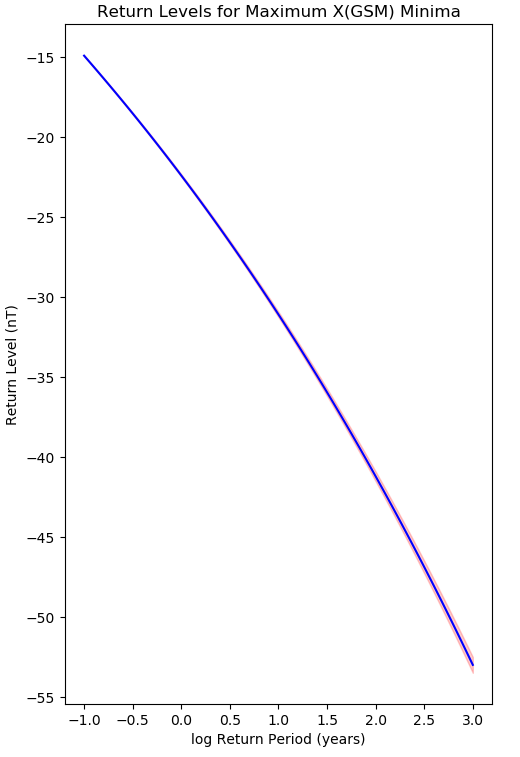
\includegraphics[width=\textwidth]{fig_method/MFImaxXminReturn.png}
                \caption{Return Level against $log_{10}$ Return Period graph of the IMF strength in the x-direction, during maximum solar activity.}
                \label{fig:MFImaxXminReturn}
            \end{minipage}
        \end{figure}
        \begin{figure}[t!]
            \begin{minipage}{0.48\textwidth}
                \centering
                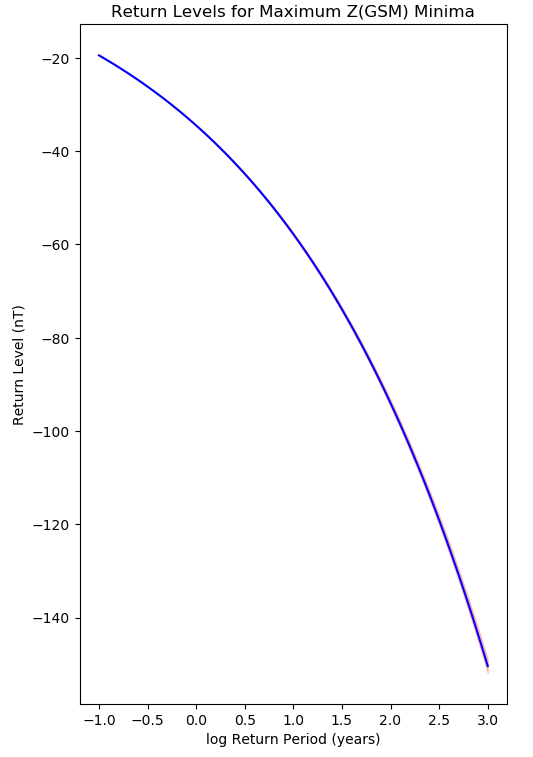
\includegraphics[width=\textwidth]{fig_method/MFImaxZminReturn.png}
                \caption{Return Level against $log_{10}$ Return Period graph of the IMF strength in the z-direction, during maximum solar activity.}
                \label{fig:MFImaxZminReturn}
            \end{minipage}
            \hfill
            \begin{minipage}{0.48\textwidth}
                \centering
                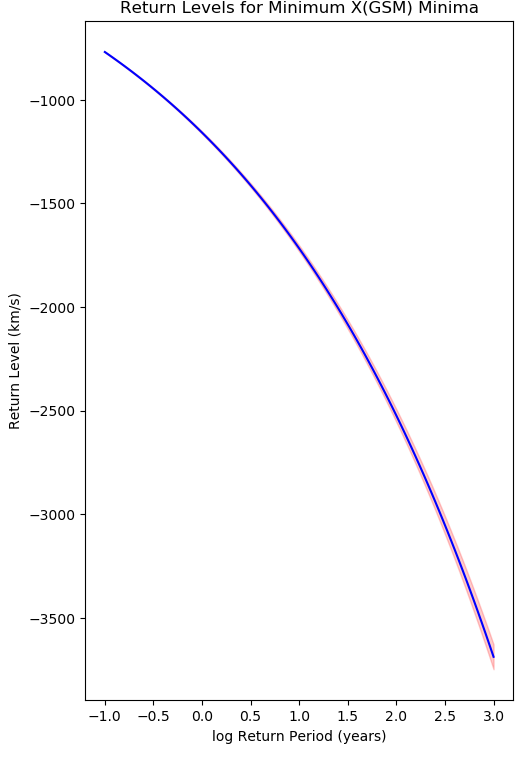
\includegraphics[width=\textwidth]{fig_method/SWEminXminReturn.png}
                \caption{Return Level against $log_{10}$ Return Period graph of the solar wind speed in the x-direction, during minimum solar activity.}
                \label{fig:SWEminXminReturn}
            \end{minipage}
        \end{figure}
        \begin{figure}[t!]
            \begin{minipage}{0.48\textwidth}
                \centering
                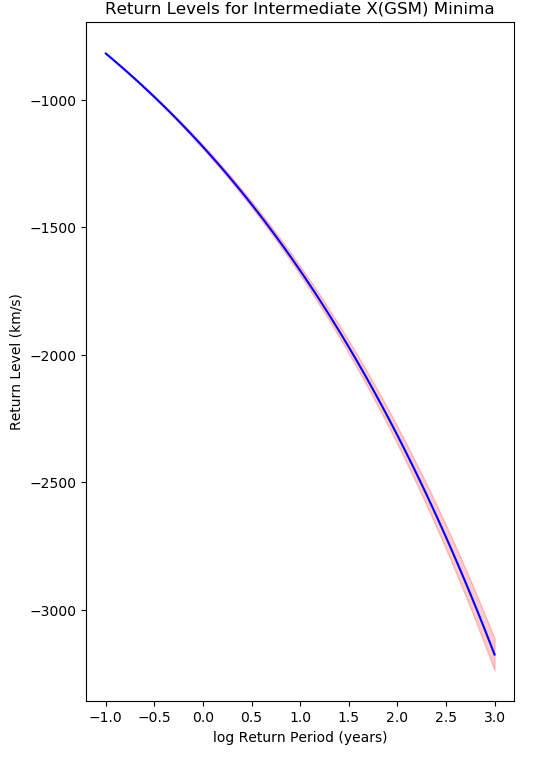
\includegraphics[width=\textwidth]{fig_method/SWEintXminReturn.png}
                \caption{Return Level against $log_{10}$ Return Period graph of the solar wind speed in the x-direction, during intermediate solar activity.}
                \label{fig:SWEintXminReturn}
            \end{minipage}
            \hfill
            \begin{minipage}{0.48\textwidth}
                \centering
                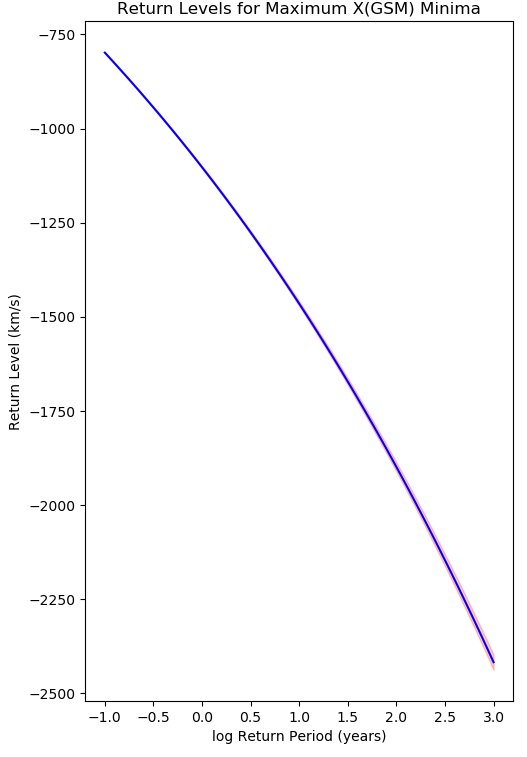
\includegraphics[width=\textwidth]{fig_method/SWEmaxXminReturn.png}
                \caption{Return Level against $log_{10}$ Return Period graph of the solar wind speed in the x-direction, during maximum solar activity.}
                \label{fig:SWEmaxXminReturn}
            \end{minipage}
        \end{figure}
        To produce return level against return period graphs, a range of return periods between 0.1 year and 1000 years has been produced and the return level for each of these return periods has been calculated and plotted. The process was repeated for each graph shown in Section \ref{sec:dailydist}.
        Since during data processing daily maxima/minima have been used, the return period has to be substituted in to the equation below, in days:
        \begin{equation}
            z_p = \mu-\frac{\sigma}{\xi}\Bigg( 1-\Bigg( -ln\Bigg( 1-\frac{1}{r}\Bigg) \Bigg) ^{-\xi}\Bigg)
        \end{equation}
        or
        \begin{equation}
            z_p = \mu-\frac{\sigma}{\xi}\Bigg( 1-\Bigg( -ln\Bigg( 1-\frac{1}{365*R}\Bigg) \Bigg) ^{-\xi}\Bigg)
        \end{equation}
        where the $z_p$ (or $-z_p$ for daily minima) is the return level, $r$ is the return period in days, $R$ is the return period in years, and $\xi$, $\mu$ and $\sigma$ are the shape, location and scale parameters respectively. From this equation, an equation for the return period in terms of the return level can be derived:
        \begin{equation}
            r=\frac{1}{1-exp\Bigg( -(1+\xi \frac{z_p-\mu}{\sigma})^{-\frac{1}{\xi}}\Bigg) }
        \end{equation}
        or
        \begin{equation}
            R=\frac{1/365}{1-exp\Bigg( -(1+\xi \frac{z_p-\mu}{\sigma})^{-\frac{1}{\xi}}\Bigg) }
        \end{equation}
        where the symbols used are described above.\\ \\
        The graphs on Figures \ref{fig:MFIintXminReturn} and \ref{fig:MFImaxXminReturn} describe the relationship between the return levels and the return periods of the IMF in the x-direction, during intermediate and maximum solar activity, respectively. As shown on these graphs, an unexpected result appears, when the two graphs are compared: The behaviour of the IMF strength in the x-direction appears to be more extreme during intermediate solar activity, than during maximum solar activity. At first thought, this might be a surprising result, but upon further inspection, two points can be made to support these results: the solar wind speed is more extreme at lower solar activity (more on this later) and the strength of the IMF depends on the speed of the solar wind, due to Alfvén's Theorem\cite{1976alfven}.\\ \\
        The graph on Figure \ref{fig:MFImaxZminReturn} describes the relationship between the return level and the return period of the IMF in the z-direction, during maximum solar activity. It is difficult to compare this graph to any of the other graphs in this section, since this is the only graph displaying properties in the z-direction.\\ \\
        The graphs on Figures \ref{fig:SWEminXminReturn}, \ref{fig:SWEintXminReturn} and \ref{fig:SWEmaxXminReturn} describe the relationship between the return levels and the return periods of the solar wind speed in the x-direction, during minimum, intermediate and maximum solar activity, respectively. The results of the comparison between these graphs has been expected, as the lower the solar activity, the more coronal holes can be found on the surface of the Sun and therefore, fast solar wind will be more abundant during lower solar activity. This means more extreme behaviour can be seen on Figure \ref{fig:SWEminXminReturn}, than on Figure \ref{fig:SWEintXminReturn} or \ref{fig:SWEmaxXminReturn}.\\
        \begin{figure}[t!]
            \begin{minipage}{0.48\textwidth}
                \centering
                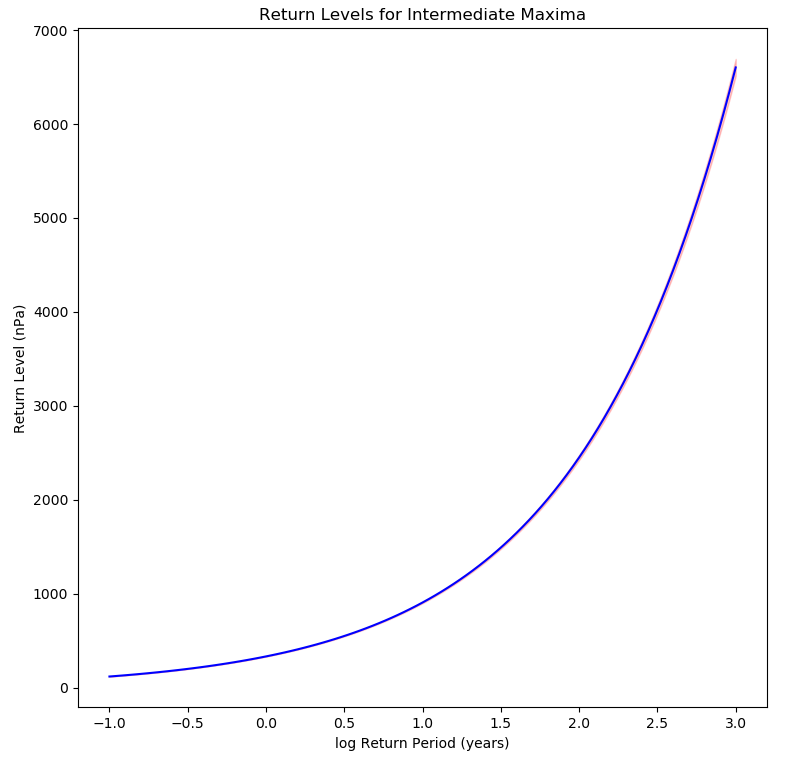
\includegraphics[width=\textwidth]{fig_method/PintmaxReturn.png}
                \caption{Return Level against $log_{10}$ Return Period graph of the solar wind ram pressure, during intermediate solar activity.}
                \label{fig:PintmaxReturn}
            \end{minipage}
            \hfill
            \begin{minipage}{0.48\textwidth}
                \centering
                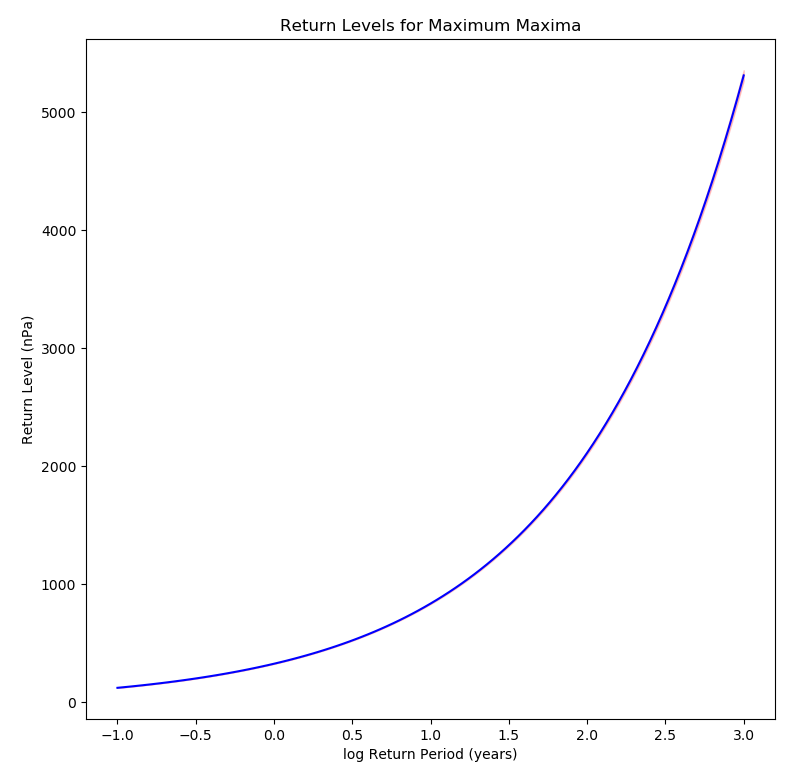
\includegraphics[width=\textwidth]{fig_method/PmaxmaxReturn.png}
                \caption{Return Level against $log_{10}$ Return Period graph of the solar wind ram pressure, during maximum solar activity.}
                \label{fig:PmaxmaxReturn}
            \end{minipage}
        \end{figure}\\
        The graphs on Figures \ref{fig:PintmaxReturn} and \ref{fig:PmaxmaxReturn} describe the relationship between the return levels and the return periods of the solar wind ram pressure, during intermediate and maximum solar activity, respectively. As the solar wind ram pressure is directly proportional to the square of the solar wind speed ($V^2$), it is expected, that the graph showing the behaviour of the solar wind ram pressure during intermediate solar activity will be more extreme. This is shown of these figures, as for a given return period, Figure \ref{fig:PintmaxReturn} gives a larger return level, than Figure \ref{fig:PmaxmaxReturn}.\\ \\
\section{Discussion}\label{sec:discussion}
    \subsection{Reaction Time for Measurements at L1 Lagrange Point}
        When preparing to take action in case the satellite at the L1 point detects high speed solar wind or a strong magnetic field, it is important to know the response time available from the moment of detection. To estimate the response time available, the time taken for the solar wind to travel from the L1 point to the satellites or the surface of the Earth needs to be calculated. Since most of the satellites orbit the Earth at a height of a few thousand kilometres, the time it takes for the high speed solar wind to travel from the L1 point to the Earth and the time it takes for it to travel from the L1 point to most satellites orbiting Earth will be approximately the same.\\ \\
        The distance between the Earth and the L1 point is approximately $1.5$ million km $ = 1.5*10^9\,$m. From Table \ref{tab:slowfast}, the minimum speed of fast solar wind is around $400\,$km/s, while in extreme cases, it can be a lot faster, than that. A prime example for a geomagnetic disturbance causing damage is the Halloween Storms in 2003. Using the data set described in Section \ref{sec:data}, the maximum speed of the solar wind during the 2003 Halloween Storms was approximately $870\,$km/s $ = 8.7*10^5\,$m/s in the negative x-direction, towards the Earth.\\ \\
        Therefore, in case of the 2003 Halloween Storms, it took the solar wind:
        \begin{equation}
            t=\frac{s}{v}=\frac{1.5*10^9}{8.7*10^5}\approx 1700\,s\approx 29\ minutes
        \end{equation}
        to reach Earth. As seen on Figure \ref{fig:hist_sw}, the solar wind speed can (very rarely) increase to approximately $1200km/s$. At this speed, the reaction time would decrease to:
        \begin{equation}
            t=\frac{s}{v}=\frac{1.5*10^9}{1.2*10^6}\approx 1250\,s\approx 21\ minutes
        \end{equation}
        assuming constant solar wind speed. This means, that governments and affected companies would have approximately 20-30 minutes to react to approaching geomagnetic storms.
    \subsection{Estimating the Return Period of a 'Carrington Event'-like Geomagnetic Storm}\label{sec:carrington}
        As return levels will have different return periods depending on the solar activity level, the following formula has been used to calculate the average of these return periods and determine the final return period for a given return level:
        \begin{equation}
            \frac{3}{R}=\frac{1}{R_{minimum}}+\frac{1}{R_{intermediate}}+\frac{1}{R_{maximum}}
        \end{equation}
        where R is the averaged return period, $R_{minimum}$ is the return period during minimum solar activity, $R_{intermediate}$ is the return period during intermediate solar activity and $R_{maximum}$ is the return period during maximum solar activity.\\ \\
        The Carrington Event is 1859 is estimated to be the largest geomagnetic storm ever recorded. At the time, direct measurements could not be made, due to lack of technology, therefore, several estimations are available about different properties of this event, based on measurements made of Earth. One article cites\cite{2013cliver} estimates that the solar wind speed reached $V_x=-1850\,$km/s and the southwards IMF strength reached $B_z\approx -65\,$nT. These estimations are also shown on Figure \ref{fig:returncarrington}.\\
        \begin{figure}[t!]
            \centering
            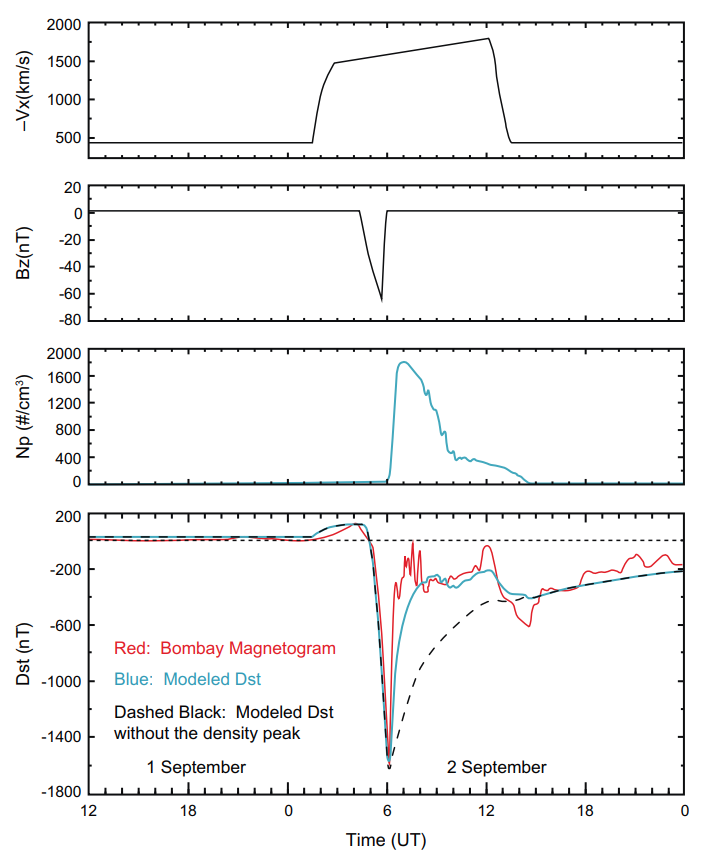
\includegraphics[width=0.7\textwidth]{fig_discussion/carrington.png}
            \caption{Approximations for the solar wind speed (top), the southward IMF strength (middle top) and the proton density (middle bottom) during the Carrington Event. Includes measurements and approximations of the disturbance storm index (Dst, bottom). As shown on the top graph, the maximum solar wind speed is approximated to be $\approx -1850\,$km/s and as shown on the middle top graph, the southward IMF strength is approximated to be $\approx 65\,$nT. Source: \cite{2006xinlin}}
            \label{fig:returncarrington}
        \end{figure}\\
        Another article\cite{2021blake} used $V_X\approx -2000\,$km/s and $B_z=-118\,$nT to simulate the Carrington Event. The differences between the estimations in these articles show, that it is nearly impossible to accurately estimate the maximum solar wind speed and the maximum southward IMF strength.\\
        Based on these 4 return levels (2 southward IMF strengths and 2 solar wind speeds), the following 4 return periods for an event comparable to the Carrington Event have been calculated:
        \begin{equation}
            \begin{split}
                B_z\cite{2013cliver}\approx -65\, nT\rightarrow R\approx 21\ years\\
                B_z\cite{2021blake}=-118\, nT\rightarrow R=317\ years\\ \\
                V_x\cite{2013cliver}=-1850\, km/s\rightarrow R=24\ years\\
                V_x\cite{2021blake}\approx -2000\, km/s\rightarrow R\approx 40\ years
            \end{split}
        \end{equation}
        As these results show, approximation and simulations to determine the maximum solar wind speed and the maximum southward IMF strength during the Carrington Event are far from perfect. The biggest outlier of these results is the approximation of the southward IMF strength of $B_z=-118\,$nT, which gives a return period of $R=317\ years$, while the other approximations all give a return period below $R=50\ years$. These results would suggest, that the true return period of an event similar to the Carrington Event would be between $R=20\ years$ and $R=317\ years$. This range of return periods does not hold any value or progress, since 20 years appears to be too small, as nothing comparable to the Carrington Event has happened since the Carrington Event itself, on the other hand, 317 years is too large, since adequate notes about geomagnetic storms before the Carrington Event do not exist and not enough time has elapsed since the Carrington Event to prove or disprove the validity of it. Therefore, the only conclusion that can be drawn for these results regarding the return period of the Carrington event, is that $20\, years < R < 317\, years$.\\ \\
        As $B_z\approx -65\, nT$ gives a return period of $R\approx20\, years$, $V_x=-1850\, km/s$ gives a return period of $R=24\, years$ and $V_x\approx -2000\, km/s$ gives a return period of $R\approx 40\, years$, it is safe to say that these values are too low to reproduce the magnetic field strength and solar wind speed expected during the Carrington Event. Therefore these estimations in article\cite{2013cliver} and in article\cite{2021blake} are too low, except for the estimation $B_z=-118\, nT$.
    \subsection{Estimating the Return Period of a 'Halloween'-like Geomagnetic Storm}\label{sec:halloween}
        The 2003 Halloween Storms is one of the largest geomagnetic storms with precisely measured properties. Measurements of different maximum values during the Halloween Storms have all been taken from the data set used in this report. The largest (smallest) values from the 2 days the storm was raging have been used (28 October 2003 and 29 October 2003). It is important to note, that measurements of solar wind speed were not available on 29 October 2003, therefore the actual solar wind speed might be more extreme, which would result in a longer return period. It has been determined, that the following extreme values characterise the 2003 Halloween Storms: $B_x=-43.6\,$nT, $V_x=-804\,$km/s, $P=54.0\,$nPa. Based on these values, the following 3 return periods for an event similar to the Halloween Storms have been calculated:
        \begin{equation}
            \begin{split}
                B_x=-43.6\, nT\rightarrow R=201\ years\\
                V_x=-804\, km/s\rightarrow R=0.11\ years\\
                P=54.0\, nPa\rightarrow R=0.022\ years
            \end{split}
        \end{equation}
        These results show a vast difference between the return periods predicted by the solar wind speed and the solar wind ram pressure and the return period predicted by the Interplanetary Magnetic Field. As the solar wind speed measurements were not available for 29 October 2003, the return periods based on the solar wind speed and the solar wind ram pressure are most likely compromised, making the return period based on the IMF strength the most reliable result. This is further enforced by the fact that the most extreme IMF strength on 28 October 2003 was $B_x=-11.3\,$nT, while on 29 October 2003, it was $B_x=-43.6\,$nT, showing a vast difference between the strength of the storm between these two days. Based only on the data collected on 28 October 2003, the return period based on the fact that $B_x=-11.3\,$nT would have been $R=0.46\ years$, which is of the same magnitude as the other, most likely compromised return periods. Due to these complications, it is safe to say that the only reliable return period is based on the IMF strength ($B_x=-43.6\,$nT), and therefore the predicted return period for an event similar to the 2003 Halloween storms is $R=201\ years$.
    \subsection{Effects of the Solar Wind on the Magnetopause of Earth}\label{sec:magnetoPAUSE}
        When the solar wind is exhibiting typical properties (displaying normal, non-extreme properties), the position of the Earth's magnetopause is determined by a delicate balance between the solar wind ram pressure and the magnetic pressure from the Earth's Magnetosphere. The formula for the solar wind ram pressure is:
        \begin{equation}
            P_{sw}=n_p*m_p*V^2
        \end{equation}
        where $n_p$ is the proton density, $m_p$ is the proton mass and $V$ is the solar wind speed. The formula for the magnetic pressure is:
        \begin{equation}
            P_{m}=\frac{B^2}{2\mu_0}
        \end{equation}
        where $\mu_0$ is the permeability of free space and $B$ is the magnetic field strength, calculated using the formula for the magnetic field of a magnetic dipole:
        \begin{equation}
            B=\frac{\mu_0m}{4\pi R^3}
        \end{equation}
        where $\mu_0$ is the permeability of free space, $m$ is the magnetic dipole moment of the Earth and $R$ is the distance from the dipole. This formula also assumes, that the point of interest is on the plane of the equator. To calculate the solar wind ram pressure needed to push the magnetopause inside the geostationary orbit, the following values have been assumed for constants and variables at the point of balance between the solar wind ram pressure and the magnetic pressure ($P_{sw}=P{m}$): $m=8.22*10^{22}\,Am^{-2}$ and $R=R_{GEO}=42164\,$km.\\ \\
        This means that the solar wind ram pressure required to push the magnetosphere inside the geostationary orbit is:
        \begin{equation}
            P_{sw}=P_{m}=4.78\, nPa
        \end{equation}
        Based on this return level, the following return period for the magnetopause being pushed inside the geostationary orbit has been calculated:
        \begin{equation}
            P=4.78\, nPa\rightarrow R=2.75*10^{-3}\ years\approx1\ day
        \end{equation}
        If the magnetic field strength at the geostationary orbit is calculated using the magnetic field strength measured on the surface of Earth (on the equator), and use the proportionality between the magnetic field strength of a magnetic dipole and the distance from said dipole ($B\propto r^{-3}$), a new estimate for the solar wind ram pressure needed can be determined:
        \begin{equation}
            P_{sw}=17.7\, nPa
        \end{equation}
        This increase in the pressure needed would mean, that the return period would increase as well:
        \begin{equation}
            P=17.7\, nPa\rightarrow R=4.09*10^{-3}\ years\approx1.5\ day
        \end{equation}
        These results of course do not consider the existence of a bow shock in front of the magnetopause, hence the solar wind ram pressure required to push the magnetopause inside the geostationary orbit is most likely reasonably higher than $P_{sw}=4.78nPa$ or $P_{sw}=17.7nPa$, which would result in a much longer return period. An assumption made so far has been that the IMF and the Earth's magnetosphere do not interact with each other. In reality, this is not the case. As the solar wind drives the IMF, it compresses the magnetosphere. The geostationary orbit is about 6.6 $R_E$ from the centre of the Earth and an article\cite{2004dimitriev} estimates that a solar wind ram pressure of 75-80 nPa is required to push the bow shock inside the geostationary orbit. This would result in the following return periods:
        \begin{equation}
            \begin{split}
                P=75\, nPa\rightarrow R=4.42*10^{-2}\ years\approx16\ days\\
                P=80\, nPa\rightarrow R=5.08*10^{-2}\ years\approx19\ days
            \end{split}
        \end{equation}
        The variation in the possible return periods shows, that the IMF-magnetosphere coupling heavily affects the amount of pressure needed to push the magnetosphere inside the geostationary orbit, and that it is therefore difficult to predict the exact return period of this pressure.
\section{Conclusion/Future Work}\label{sec:conclusions}
    In conclusion, a data set of the strength of the Interplanetary Magnetic Field and solar wind speed, measured at the L1 point has been analysed and for the purpose of creating relations between the return level and the return period of space weather events. The data sets have been separated based on solar magnetic activity level and coordinates. Then, the daily maxima (minima) of these data sets have been separated and a line of best fit was fitted on them, using Generalised Extreme Value Distribution. The most important relations included solar wind speed in the GSM x-direction, magnetic field strength in the GSM x-direction and z-direction and solar wind ram pressure. Using these relations, return level against return period graphs have been plotted to use them to estimate the return period of two well-known space weather events: the 1859 Carrington Event and the 2003 Halloween Storms.\\ \\
    Predictions for the return period of the Carrington Event gave a range of values between $R\approx 21\, years$ and $R=317\, years$, although estimations for the strength of the Interplanetary Magnetic Field and the solar wind speed during the event are sparse, due to the lack of technology during that time. These estimations are based on measurements taken on the surface of Earth and the most reliable method to estimate the magnetic field strength and the solar wind speed outside of the Earth's magnetic field was to try to recreate the event using simulations. While these simulations produce reasonable measurements, their accuracy is questionable and a small difference between the estimated values and the actual values caused the estimated return period to be somewhat questionable, imprecise and unreliable. The IMF strength and solar wind speed estimations that give the three low values for the return period of the Carrington Event are thought to be underestimating the IMF strength and the solar wind speed during the Carrington Event.\\ \\
    The return period of the Halloween Storms has been estimated to be $R=201\ years$, although this is based on only a single relation (the Interplanetary Magnetic Field strength in the GSM x-direction), as most measurements from this time were largely unavailable.\\ \\
    Another factor hindering the accurate estimation of these values was the presence of both slow and fast solar wind speed data in the same data set. This caused inaccurate and imprecise estimations for the parameters of the Generalised Extreme Value Distribution in several relations, most notable in the distribution of the solar wind speed in the x-direction, during minimum (Figure \ref{fig:SWEminXmin}) and intermediate (Figure \ref{fig:SWEintXmin}) solar activity.\\ \\
    Future work would include several ways and methods to improve the quality of data and eliminate some of the assumptions, that have been made in the context of the data and the data processing. Given data over a longer period of time, the use of daily maxima (minima) could be eliminated and the use of weekly maxima (minima) could be introduced, while keeping the number of data points the distribution functions are based on high. This would help increase the independence of these data points, as they would be temporally further apart. Another way to improve the accuracy of the relations set up between return levels and return periods using the solar wind speed would be to separate the data points referring to slow solar wind and to fast solar wind. As slow solar wind and fast solar wind have different origins/sources, they cannot be considered to be random samples from the same distribution, as slow solar wind data points and fast solar wind data points would have different distributions. Improvements could also be made on the method to determine the solar magnetic activity level at a given time, based on measurements of the state of the Heliosphere at the given time. The return period estimations could be improved by combining the the solar wind speed and the IMF strength to estimate the strength of the electric field, which might be a better way to produce return period estimations.
\newpage{}
\pagenumbering{alph}

\bibliographystyle{unsrt}
\bibliography{bibliography.bib}

\end{document}